%%=============================================================================
%% Chaos Engineering Tools
%%=============================================================================

\chapter{\IfLanguageName{dutch}{Chaos Engineering Tools}{Chaos Engineering Tools}}
\label{ch:chaostools}

Het toepassen van chaos engineering is relatief nieuw, maar er zijn ondertussen al heel wat tools op de markt verschenen om chaos experimenten te kunnen uitvoeren. De Cloud Native Computing Foundation (CNCF), een Linux Foundation project gestart in 2015, is de thuisbasis van heel wat open source projecten die vandaag het landschap definiëren in de IT-sector. CNCF projecten kunnen drie niveaus van maturiteit hebben nl. sandbox, incubating en graduated. Deze niveau's geven aan hoe ver een project geëvolueerd is. \autocite{CNCF2022a}
\newline Men kan een overzicht van deze projecten, gerangschikt per categorie, terugvinden in het CNCF Cloud Native Interactive Landscape. Eén van deze categorieën is chaos engineering, waar men  een lijst kan terugvinden van chaos engineering tools. \autocite{CloudNativeLandscape2022}

Pavlos Ratis, Site Reliability Engineer bij RedHat OpenShift, onderhoudt een Github repository  waar men heel wat zaken omtrent chaos engineering kan terugvinden. In deze repository vindt men in de sectie 'Notable Tools' een lijst van chaos engineering tools die bruikbaar zijn voor verschillende doeleinden. Deze lijst werd eveneens geraadpleegd in de zoektocht naar een geschikte tool om chaos engineering experimenten toe te passen op een Kubernetes cluster. \autocite{Ratis2022}.

De eerste tool die onderzocht werd is Chaos Toolkit, via een cursus op het online leerplatform Udemy. Nadien kwamen uit de eerder vernoemde bronnen nog twee andere tools naar boven genaamd ChaosMesh en Litmus.

Vooraleer men experimenten kan beginnen uitvoeren heeft men eerst een demo-applicatie nodig. Volgend hoofdstuk beschrijft hoe men twee demo-applicaties kan opzetten waar men later experimenten op kan toepassen. Deze identieke setup zal gerepliceerd worden telkens een chaos engineering tool besproken wordt.

Daarna komt de installatie van de verschillende chaos engineering tools en het uitvoeren van de experimenten aan bod.

\section{Demo-applicaties opzetten}

Aangezien dit onderzoek gericht is om experimenten uit te voeren voor educatieve doeleinden, is gekozen om eerst enkele experimenten uit te voeren op Nginx en Apache webserver pods. Door twee aparte Deployments en Services op te zetten kon de onderlinge communicatie tussen beiden aangetoond en getest worden. Dit was praktisch om experimenten uit te voeren waarbij de communicatie verstoord werd tussen verschillende Services, of experimenten enkel te richten op specifieke pods in een namespace. 

Het visuele aspect ontbrak hierbij echter om de impact van een experiment te verduidelijken op de applicatie in een browser. Vandaar is gekozen om enkele experimenten te herhalen op een tweede demo-applicatie genaamd PodTato-Head, een applicatie die een aardappelmannetje toont en waarbij de lichaamsdelen bestaan uit verschillende pods, opgezet via afzonderlijke Deployments en Services.   Met behulp van deze applicatie kon o.a. aangetoond worden dat een applicatie nog steeds bereikbaar kan zijn desondanks bepaalde pods getroffen worden.

Men kan alle experimenten die hieronder beschreven staan ook toepassen op de PodTato-Head applicatie door simpelweg de namespace aan te passen waar nodig naar 'demoapp2'.

\subsubsection{Demo-applicatie 1:Nginx/Apache webserver pods}

De eerste demo applicatie kan men onderbrengen in een aparte namespace genaamd demoapp1. Op deze manier kan men de impact van de experimenten (= de blast radius) beperken en voorkomen dat andere pods ongewenst mee betrokken worden in een experiment. Om de eerste demo-applicatie tot stand te brengen voert men volgende commando's uit: 
\begin{lstlisting}[language=bash]
# Creëer een nieuwe namespace voor de experimenten
$ kubectl create ns demoapp1

# Creëer een Deployment met 3 Apache pods
# in de namespace litmusexperiments
$ kubectl create deploy apache --image=bitnami/apache \
--replicas=3 -n demoapp1

# Creëer een Service voor de Apache pods
# Apache luistert in container op poort 8080
$ kubectl expose deploy apache --port=80 \
--target-port=8080 -n demoapp1

# Creëer een Deployment met 3 Nginx pods 
# in de namespace demoapp1
$ kubectl create deploy nginx --image=nginx \
--replicas=3 -n demoapp1

# Creëer een LoadBalancer Service voor de Nginx pods
$ kubectl expose deploy nginx --port=80 --type=LoadBalancer \
-n demoapp1

\end{lstlisting} 

Wanneer men vervolgens via commando {\bf kubectl get svc -n demoapp1} de Services opvraagt zal men zien dat een extern IP-adres bij de Nginx LoadBalancer Service te zien is. Via de browser kan men nu surfen naar dit IP-adres en zal men de nginx default webpagina te zien krijgen. 

\subsection{Demo-applicatie 2: PodTato-Head}
\label{subsec:podtato-setup}

De tweede demo applicatie PodTato-Head kan men onderbrengen in een aparte namespace genaamd demoapp2. De manier hoe deze geïnstalleerd wordt is opnieuw via het eerder gebruikte Helm, alhoewel men ook o.a. kubectl kan gebruiken om deze te installeren. \autocite{Gavant2022}

Maak eerst een nieuwe directory aan op het systeem waarin men in volgende stappen de PodTato-Head repository kan in bewaren. 

Men voert volgende commando's uit in de nieuwe directory om de applicatie te installeren:
\begin{lstlisting}[language=bash]
    # Creëer de namespace demoapp2
    $ kubectl create ns demoapp2
    
    # Kloon de podtato-head Git repo in de directory
    $ git clone https://github.com/podtato-head/podtato-head.git
    
    # Ga verder naar de podtato-head directory
    $ cd podtato-head/
    
    # Installeer de podtato-head app in namespace demoapp2
    $ helm install podtato-head ./delivery/chart -n demoapp2 
    
    # Verifieer als de app pods + services operationeel zijn
    $ kubectl get pods -n demoapp2
    $ kubectl get svc -n demoapp2
\end{lstlisting} 

Via de output van het 'helm install ...' commando ziet men enkele commando's hoe de URL verkregen kan worden om toegang tot de applicatie te bekomen via de browser.  \newline Zie figuur \ref{img:podtato-head} als voorbeeld hoe de applicatie er in de browser uitziet. 

\begin{figure}[h]
    \centering
    
\includegraphics[scale=.5]{img/podtatohead-app.png}
    \caption{Podtato-Head applicatie}
    \label{img:podtato-head}
\end{figure}

Nota: Bovenstaande output bevat een LoadBalancer Service, maar in geval de applicatie in een lokale omgeving geïnstalleerd wordt zal hier een NodePort of ClusterIP te zien zijn. In dat geval zal men andere stappen moeten ondernemen om de toegang tot de applicatie in de browser te bekomen. 
Zie sectie {\bf Test the API Endpoint} in de bron die aan het begin van dit hoofdstuk vermeld wordt, waar de nodige acties omschreven worden om toe te passen in deze verschillende situaties.  

\section{Chaos Toolkit}

De eerst besproken chaos engineering tool in dit onderzoek is Chaos Toolkit. Deze tool kwam aan bod in de Udemy cursus 'Kubernetes Chaos Engineering With Chaos Toolkit and Istio' en was volgens \textcite{Viktor Farcic}, de lesgever en auteur van het gelijkaardig genaamd boek, de beste chaos engineering tool op dat moment (maart 2020) beschikbaar. 

Er zullen in dit onderzoek enkele eenvoudige experimenten aan bod komen, zowel uitgevoerd op de applicatie in namespace demoapp1 als demoapp2, die de verschillende componenten van Chaos Toolkit en de algemene werking ervan zullen omschrijven. Vooraleer hiermee van start te gaan zal eerst beschreven worden hoe deze tool geïnstalleerd wordt.    

\subsection{Installatie Chaos Toolkit}

De enige vereiste wanneer men ChaosToolkit wil installeren is dat Python op het systeem nodig is. \autocite{ChaosToolkit2022b}

Voor een Linux Debian/Ubuntu distributie kan men volgend commando gebruiken om de nodige packages te installeren: {\bf sudo apt-get install python3 python3-venv}
 
ChaosToolkit zal geïnstalleerd worden in een Python virtuele omgeving. Dit is een geïsoleerde omgeving die toelaat om afzonderlijke afhankelijkheden te beheren voor verschillende Python projecten. \autocite{UniMinnesota2022}

Gebruik volgend stappenplan om Chaos Toolkit te installeren in de Google Cloud Shell. Dezelfde werkwijze kan men ook toepassen in een lokale omgeving.
\begin{lstlisting}
# Maak een virtuele omgeving aan
$ python3 -m venv ~/.venvs/chaostk

# Activeer deze virtuele omgeving
$ source  ~/.venvs/chaostk/bin/activate

# Installeer de CLI
$ pip install -U chaostoolkit

# Verifieer succesvolle installatie CLI
$ chaos --version
\end{lstlisting}

Chaos Toolkit is nu geïnstalleerd in de virtuele omgeving op het systeem. Dit kan men zien doordat links naast de username nu (chaostk) zal te zien zijn. 
{\bf Let op:} Wanneer men de sessie beëindigd door de terminal te sluiten zal men eveneens deze virtuele omgeving verlaten. Wanneer men opnieuw richting deze omgeving wil gaan dient men het commando {\bf source  ~/.venvs/chaostk/bin/activate} nogmaals uit te voeren. Vergeet men dit echter te doen dan zal het 'chaos' commando niet gevonden worden wanneer men dit in de terminal probeert uit te voeren, aangezien dit commando enkel in de geïsoleerde virtuele omgeving bestaat.

Chaos Toolkit bevat na installatie voorlopig weinig functionaliteit. Men kan namelijk op dit moment nog geen experimenten opzetten die toepasbaar zijn op een Kubernetes cluster. Om dit mogelijk te maken dient men de {\bf chaostoolkit-kubernetes} plugin te installeren. \autocite{ChaosToolkit2022}. 
Via volgende stappen kan men eerst de chaostoolkit-kubernetes plugin installeren op het systeem en vervolgens de verschillende experimentconfiguraties opvragen die deze plugin bevat.
\begin{lstlisting} 
# Installeer chaostoolkit-kubernetes plugin
$ pip install chaostoolkit-kubernetes

# Creëer bestand 'discovery.json' met overzicht qua opties
$ chaos discover chaostoolkit-kubernetes

# Ontdek alle opties voor experimenten in Kubernetes
$ cat discovery.json
\end{lstlisting}

Andere extensies/plugins waarmee men de functionaliteit van Chaos Toolkit verder kan uitbreiden om bv. experimenten op te zetten m.b.t. specifieke cloudarchitecturen en platformen, netwerkgerelateerde experimenten ... kan men via volgende link raadplegen: \url{https://github.com/search?utf8=%E2%9C%93&q=topic%3Achaostoolkit-extension&type=Repositories} 

\subsection{Een experiment opzetten}

Chaos Toolkit is CLI-gebaseerd, wat wil zeggen dat experimenten enkel via de terminal uitgevoerd kunnen worden. Voorgedefinieerde experimenten worden niet aangeboden bij deze tool, maar de bedoeling is om de experimenten modulair op te bouwen door de afzonderlijke componenten hieronder beschreven in een YAML- of JSON-bestand te definiëren \autocite{ChaosToolkit2022a}:
\begin{enumerate}
    \item {\bf Beschrijving experiment}: versie, titel, tags.
    \item {\bf De 'steady-state-hypothesis'}: De hypothese waarin men een controle (= probe) definieert om het normale gedrag (= de steady state) te valideren.
    \item {\bf Een 'method'}: De activiteiten van een chaos experiment. Deze kunnen acties en probes bevatten die omschrijven hoe het experiment moet uitgevoerd worden.  
    \item {\bf Een 'rollback'}: Het chaos experiment ongedaan maken en terugkeren naar een normale staat. Nota: Een Kubernetes cluster bevat alreeds enkele zelfhelende eigenschappen waardoor een rollback configureren hierbij soms onnodig is.
\end{enumerate}
    
Men kan zelf kiezen om deze YAML- of JSON-definitie te creëeren, maar via commando {\bf chaos init} kan men ook een experiment opzetten waarbij de verschillende stappen in het proces met begeleiding van een wizard afgerond kunnen worden. 

Experimenten die via de wizard opgezet worden leiden tot de creatie van een {\bf experiment.json} bestand. Wanneer men op dezelfde manier een nieuw experiment wil opzetten zal dit JSON-bestand overschreven worden. Men kan dit echter voorkomen door zelf een naam mee te geven in dit commando. Eveneens heeft men de optie om als output een YAML-bestand te bekomen. Zowel de naam van het experiment als de keuze qua configuratietaal bekomt men via commando {\bf chaos init --experiment-path [experiment naam].[json | yaml]}.

Er zal ook een {\bf journal.json} bestand gecreëerd worden na de uitvoer van een experiment opgezet via het 'chaos init' commando. Dit toont o.a. de definitie van het uitgevoerde experiment, welke pods getroffen zijn, wanneer en hoelang het experiment uitgevoerd is ...
Alleen het laatst uitgevoerde experiment wordt bewaard in dit bestand m.a.w. ook dit wordt overschreven bij elke uitvoer van een nieuw experiment.   

Zowel de setup m.b.v. de wizard via het 'chaos init' commando, alsook het zelf creëeren van experiment-definities zullen in komende experimenten beschreven worden. Vooraleer men van start gaat met het experimenteren maakt men een nieuwe directory waarin deze experimenten zullen bewaard worden genaamd 'chaostoolkit-experiments' m.b.v. commando {\bf mkdir chaostoolkit-experiments}. 

\subsection{Experiment 1: Een random pod vernietigen}

In dit experiment zal een willekeurige nginx pod van de demoapplicatie in namespace demoapp1 vernietigd worden. De bedoeling is om te zien hoe het systeem zal reageren wanneer een pod vernietigd wordt. Aangezien de pods in de demoapp1 namespace via een Deployment zijn opgezet, zou het vernietigen van een pod steeds de ReplicaSet moeten triggeren om een nieuwe pod te creëeren.

Zet het experiment op volgende manier op:  
\begin{enumerate}
    \item Ga naar de chaostoolkit-experiments directory en voer commando {\bf chaos init} uit.
    \item Geef een naam aan het experiment vb. random-pod-kill.
    \item Geef deze keer géén steady-state hypothese op. Dit zal in volgende experimenten aan bod komen.
    \item Antwoord met 'y' op de vraag 'Do you want to define an experimental method?' Dit zal een lijst weergeven met alle mogelijke acties die uitgevoerd kunnen worden. 
    \item Kies de actie 'terminate\textunderscore pods' in deze lijst (= optie 26) en bevestig de keuze met 'y'. 
    \item Vervolgens zal men enkele parameters moeten opgeven voor deze actie: 
    \begin{enumerate}
        \item {\bf label\textunderscore selector}: geef hier 'app=nginx' in om het experiment op de nginx te richten.
        \item {\bf name\textunderscore pattern}: via enter kiest men de defaultwaarde 'null'.
        \item {\bf all}: via enter kiest men de defaultwaarde 'False' om aan te geven dat niet alle pods moeten vernietigd worden.
        \item {\bf rand}: geef 'True' in, om een willekeurige pod te selecteren.
        \item {\bf mode}: via enter kiest men de defaultwaarde 'Fixed'
        \item {\bf qty}: via enter kiest men de defaultwaarde '1', wat neerkomt op het aantal pods die vernietigd moet worden.
        \item {\bf grace\textunderscore period}: via enter kiest men de defaultwaarde '-1' wat overeenkomt met onmiddelijke vernietiging van de pod.
        \item {\bf ns}: geef hier de namespace 'demoapp1' op.
        \item {\bf order}: via enter kiest men de defaultwaarde 'Alphabetic'.
    \end{enumerate}
    \item Antwoord met 'N' op de vraag 'Do you want to select another activity?' om aan te geven dat geen extra acties meer ondernomen moeten worden in dit experiment.
\end{enumerate} 

De wizard is afgelopen en het bestand 'experiment.json' zal vervolgens gecreëerd worden in deze directory. Men kan dit experiment uitvoeren via commando {\bf chaos run experiment.json}
De uitvoer van het experiment in onderstaande output toont aan dat dit succesvol verlopen is:
\begin{lstlisting}
$ chaos run experiment.json
[INFO] Validating the experiment's syntax
[INFO] Experiment looks valid
[INFO] Running experiment: random-pod-kill
[INFO] Steady-state strategy: default
[INFO] Rollbacks strategy: default
[INFO] No steady state hypothesis defined. 
[INFO] Playing your experiment's method now...
[INFO] Action: terminate_pods
[INFO] Let's rollback...
[INFO] No declared rollbacks, let's move on.
[INFO] Experiment ended with status: completed
\end{lstlisting}

Men ziet in de uitvoer dat dit experiment geen steady-state probeert te bevestigen of een rollback uitvoert, maar louter één actie 'terminate\textunderscore pods' doorloopt.
Indien bovenstaande regels enkel groen gekleurd zijn kan men concluderen dat het experiment zonder fouten doorlopen is. De kleur van deze regels kan ook oranje of rood zijn bij afwijkingen tijdens de uitvoer van het experiment, maar dit zal vaker voorkomen bij het valideren van de steady state bv. door een probe die faalt.  
 
Via het commando {\bf cat journal.json} kan men de details opvragen van het uitgevoerde experiment zoals de definitie van het experiment, de start- en eindtijd, de getroffen pod , de status ... 

Tijdens de uitvoer van dit experiment kan men via commando {\bf k9s -n demoapp1} zien hoe één van de nginx pods in de namespace demoapp1 vernietigd wordt (zie kolom Status) en hoe direct daarna een nieuwe pod gecreëerd wordt om terug tot drie actieve pods te komen. 

\begin{figure}[h]
    \centering
    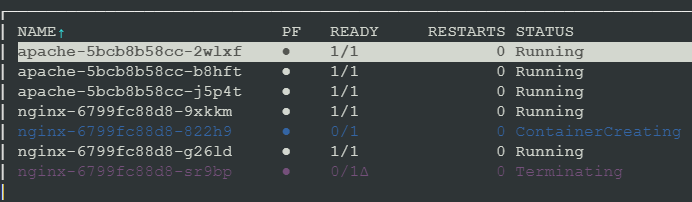
\includegraphics{img/k9s-chaostoolkit-ex1.png}
    \caption{k9s uitvoer van Chaos Toolkit experiment 1}
    \label{img:chaostoolkitexperiment1}
\end{figure}

Men hoeft de configuratie niet noodzakelijk te bekomen via het 'chaos init' commando maar kan een experiment ook opzetten via een vooraf gedefinieerd YAML-bestand. Via volgende stappen zet men dit op: 
\begin{enumerate} 
    \item Creëer een nieuw bestand genaamd 'random-pod-kill.yaml' m.b.v. een teksteditor naar keuze. 
    \item Klik op volgende link naar de Github repository waar men een YAML-definitie voor dit experiment kan terugvinden: \href{https://github.com/KenBruggeman/BP\textunderscore 21-22/blob/master/bachelorproef/docs/chaostoolkit%20experimenten/random-pod-kill.yaml}{Experiment 1: random-pod-kill.yaml}
    \newline Men ziet in dit bestand eerst een beschrijving van het experiment, gevolgd door de configuratie van de 'method'. Ook hier ontbreekt dus de configuratie van andere componenten zoals een steady state of een rollback, die in volgende experimenten nog aan bod zullen komen.
    \item Neem de inhoud van dit bestand over in het nieuw gecreëerde bestand random-pod-kill.yaml en sla op.
    \item Herhaal het experiment m.b.v. deze YAML-definitie via commando {\bf chaos run random-pod-kill.yaml}.
\end{enumerate}

\subsection{Experiment 2: uitbreiding experiment 1 met steady state}

In dit experiment zal experiment 1 aangevuld worden met een Steady State Hypothesis, die voor en na het verwijderen van een willekeurige nginx pod het aantal nginx pods zal controleren.

Eerst zal men de stappen via de wizard nogmaals doorlopen om dit experiment op te zetten maar deze keer zal gevraagd worden een YAML-definitie als output te bekomen. Dit doet men via commando {\bf chaos init --experiment-path random-pod-kill-ssh.yaml} (ssh = steady state hypothesis)
Start de setup van dit experiment via commando {\bf chaos init}. Configureer volgende zaken via de wizard:
\begin{enumerate}
    \item {\bf Experiment's title:} random-pod-kill-ssh
    \item Antwoord met {\bf 'y'} op de vraag 'Do you want to define a steady state hypothesis now?'
    \item {\bf Hypothesis's title:} Er zijn drie nginx pods aanwezig
    \item {\bf Add an activity:} geef het nummer op van de optie 'count\textunderscore pods'.
    \item Antwoord met {\bf 'y'} op de vraag 'Do you want to use this probe?'
    \item {\bf What is the tolerance for this probe?:} 3 (= het aantal nginx pods in de applicatie)
    \item {\bf label\textunderscore selector:} app=nginx
    \item {\bf phase:} via enter kiest men de default [].
    \item {\bf ns:} demoapp1
    \item Antwoord met {\bf 'N'} op de vraag 'Do you want to select another activity?'. Hiermee vraagt men namelijk als nog een andere controle in een tweede 'steady state hypothesis' moet gecreëerd worden. 
    \item Antwoord met {\bf 'y'} op de vraag Do you want to define an experimental method?'
    \item Resterende configuratie vanaf {\bf label\textunderscore selector} is dezelfde als bij experiment 1.
\end{enumerate}

{\bf Let op:} Wanneer men de zopas gecreëerde 'random-pod-kill-ssh.yaml' gaat bekijken zal men zien dat onder de configuratie bij {\bf probes} bij de parameter {\bf tolerance} single quotes rond de waarde 3 zullen staan. De kans is groot dat hierdoor de uitvoer van het experiment zal falen dus verwijder deze quotes en sla het bestand terug op. Het experiment uitvoeren doet men vervolgens via commando {\bf chaos run random-pod-kill-ssh.yaml}.
  
In figuur \ref{img:chaostoolkitex2} ziet men dat zowel voor als na de Action 'terminate-pod' de probe uitgevoerd wordt. Wanneer men dit experiment reproduceert zal de probe hoogstwaarschijnlijk na de actie terug falen met de melding: 'Steady state probe 'count\textunderscore pods' is not in the given tolerance so failing this experiment'.
\newline Dit komt omdat de probe direct na de actie uitgevoerd werd en er dus onvoldoende tijd werd gegeven aan Kubernetes om een nieuwe pod op te starten.

\begin{figure}[h]
    \centering
    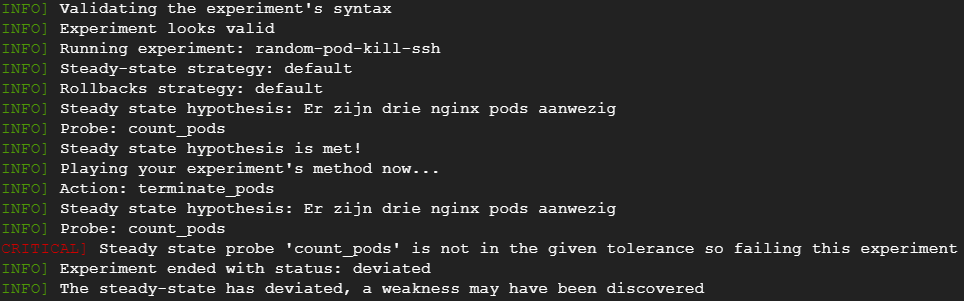
\includegraphics[scale=.7]{img/chaostoolkit-ex2.png}
    \caption{Probe faalt bij uitvoer Chaos Toolkit experiment 2}
    \label{img:chaostoolkitex2}
\end{figure}

Als oplossing kan men een parameter {\bf pauses} aan de configuratie toevoegen zodat na de actie enkele seconden gewacht wordt vooraleer opnieuw de controle uit te voeren. Deze parameter pauses kan men echter niet configureren via de chaos init wizard maar zal manueel toegevoegd moeten worden.
Men kan gebruik maken van volgend voorgedefinieerd YAML-bestand om de configuratie over te nemen en het experiment te herhalen: \href{https://github.com/KenBruggeman/BP\textunderscore 21-22/blob/master/bachelorproef/docs/chaostoolkit%20experimenten/random-pod-kill-ssh.yaml}{Experiment 2: random-pod-kill-ssh.yaml}
    
\subsection{Experiment 3: uitbreiding vorige experimenten}

Door de tekortkomingen die in vorig experiment bewezen werden bij de experimentconfiguratie via het 'chaos init' commando zal in volgende experimenten louter nog gebruik gemaakt worden van een voorgedefinieerd YAML-bestand. 

De parameter {\bf qty} wordt in dit experiment geïntroduceerd waarmee men vorig experiment kan uitbreiden zodat meerdere pods in de namespace demoapp1 vernietigd kunnen worden. Eveneens zal gebruik gemaakt worden van een andere probe genaamd {\bf pods\textunderscore in\textunderscore phase} die de status van de pods zal controleren i.p.v. het aantal pods te tellen. De defaultwaarde van deze probe is ingesteld op 'Running' dus hoeft dit niet noodzakelijk in de configuratie opgenomen te worden. \autocite{ChaosToolkit2022c}

Volgende stappen kan men toepassen om het experiment op te zetten en uit te voeren:
\begin{enumerate}
    \item Creëer een nieuw YAML-bestand genaamd 'multiple-random-pod-kill-ssh.yaml'. 
    \item Kopieer de definitie van dit experiment die men kan terugvinden via volgende link: \href{https://github.com/KenBruggeman/BP\textunderscore 21-22/blob/master/bachelorproef/docs/chaostoolkit%20experimenten/multiple-random-pod-kill-ssh.yaml}{Experiment 3: multiple-random-pod-kill-ssh.yaml}
    \item Voer dit experiment uit m.b.v. commando {\bf chaos run multiple-random-pod-kill-ssh.yaml} 
\end{enumerate}

De YAML-definitie van dit experiment ontbreekt een waarde bij parameter {\bf label\textunderscore selector} waardoor nu alle pods in de namespace demoapp1 getroffen kunnen worden. Men ziet via de k9s tool dat bij het uitvoeren van dit experiment hierdoor nu ook de Apache pods getroffen worden. De slaagkans van de probe na de actie 'terminate\textunderscore pods' is afhankelijk van de snelheid waarmee Kubernetes de nieuwe pods kan creëeren.  

\subsection{Experiment 4: bereikbaarheid van Podtato-Head applicatie testen}

In dit experiment zal de demo-applicatie Podtato-Head in namespace demoapp2 gebruikt worden. Deze applicatie is alreeds opgezet in hoofdstuk \ref{subsec:podtato-setup} en men kon daar alreeds de URL te zien krijgen waarop de applicatie bereikbaar is. Deze URL zal men nodig hebben in de configuratie van het experiment.

Dit experiment zal het gevolg testen van het vernietigen van pod 'podtato-head-entry', die verantwoordelijk is voor de toegang tot de applicatie. Voor en na de vernietiging van deze pod zal via een {\bf http probe} gecontroleerd worden als de applicatie terug bereikbaar is. \autocite{ChaosToolkit2022d}
 
Men kan in deze probe een parameter {\bf timeout} configureren en een waarde meegeven hoelang het maximum mag duren om een antwoord op de GET-request te krijgen. Als antwoord wordt een HTTP-response status code 200 verwacht, wat wil zeggen dat de applicatie bereikbaar is. Alternatief kunnen ook twee waardes als JSON array geconfigureerd worden waarbij de eerste waarde de connection timeout weergeeft,
en de tweede waarde de request timeout. Meer info over deze twee types timeout kan men in volgende link terugvinden: \href {https://stackoverflow.com/questions/49704708/what-is-a-connection-timeout-during-a-http-request}{what-is-a-connection-timeout-during-a-http-request}

Gebruik volgend stappenplan om dit experiment op te zetten:
\begin{enumerate}
  \item Creëer een nieuw YAML-bestand genaamd 'podtato-entry-kill-httpprobe.yaml'.
  \item Kopieer de definitie in volgende link om dit bestand op te vullen:
  \href{https://github.com/KenBruggeman/BP\textunderscore 21-22/blob/master/bachelorproef/docs/chaostoolkit%20experimenten/podtato-entry-kill-httpprobe.yaml}{Experiment 4: podtato-entry-kill-httpprobe.yaml}
  \item Pas de parameter {\bf url} aan naar deze die men bij de setup van de Podtato-Head applicatie in hoofdstuk \ref{subsec:podtato-setup} alreeds heeft bekomen.
  \item Sla de wijzigingen op.
  \item Voer het experiment uit via commando {\bf chaos run podtato-entry-kill-httpprobe.yaml}.
\end{enumerate} 

\\ \newline Het resultaat van dit experiment ziet men in figuur \ref{img:chaostoolkitex4}. Ondanks een pauze van tien seconden faalt de probe na de actie nog steeds. Op deze manier kan men zien dat de applicatie meer tijd nodig heeft vooraleer deze terug bereikbaar is.

\begin{figure}[h]
    \centering
    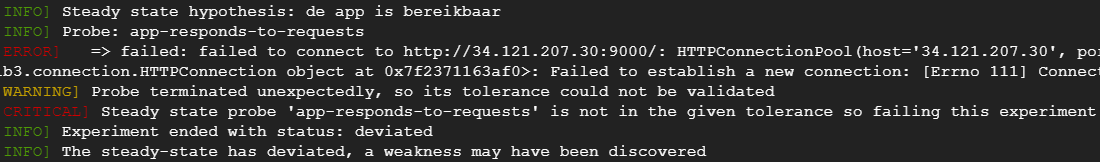
\includegraphics[width=15cm, height=4cm]{img/chaostoolkit-ex4.png}
    \caption{http probe faalt bij uitvoer Chaos Toolkit experiment 4}
    \label{img:chaostoolkitex4}
\end{figure}

\\ {\bf Oplossing:} Een applicatie die onbereikbaar is wil men ten allen tijde vermijden. Wat men ziet in de Podtato-Head applicatie is dat elke pod slechts één keer voorkomt. In deze applicatie wordt elke pod voorzien door een aparte Deployment. Een voordeel van pods die opgezet worden via een Deployment is dat deze makkelijk te schalen zijn.
Als oplossing op voorgaand gefaald experiment kan men dus de Deployment die verantwoordelijk is voor de podtato-head-entry pod schalen zodat deze steeds twee pods actief heeft. Als één pod in de problemen komt zal de andere de bereikbaarheid van de applicatie toch nog verzekeren. 
Men kan dit controleren via commando {\bf kubectl get deploy -n demoapp2}. In de output van dit commando ziet men dat de Deployment eveneens podtato-head-entry noemt. Om deze te schalen zodat steeds twee pods actief zijn past men volgend commando toe: {\bf kubectl scale deploy podtato-head-entry --replicas=2 -n demoapp2}. Als gevolg kan men zien via de k9s tool dat een extra podtato-head-entry pod gecreëerd is in namespace demoapp2.

Herhaal vervolgens het experiment en als resultaat zal men nu zien dat de applicatie bereikbaar blijft wanneer één van de podtato-head-entry pods getroffen wordt. Als test kan men de parameter pauses in commentaar plaatsen in de YAML-definitie, zodat de http probe rechtstreeks na de actie uitgevoerd wordt.  

\subsection{Referenties toepassen in een experiment}

Wanneer men een actie of probe opnieuw wil uitvoeren dan kan men via een referentie verwijzen naar de alreeds bestaande configuratie van die actie of probe. Zie als voorbeeld de onderstaande code uit de YAML-definitie van experiment 4 waarin een probe herhaald wordt door ernaar te refereren via parameter {\bf ref}:  

\begin{lstlisting}[language=bash] 
steady-state-hypothesis:
  title: Applicatie is bereikbaar
  probes:
  - name: response-OK
    type: probe
    tolerance: 200
    provider:
      type: http
      timeout: [1,2]
      verify_tls: false
      url: http://34.121.207.30:9000/
  - type: probe 
    tolerance: 200
    ref: response-OK
\end{lstlisting}

Ter info: Men hoeft een probe niet noodzakelijk in een steady-state-hypothesis te definiëren. Wil men  een probe tijdens de actie van het experiment uitvoeren dan kan men dit in de 'method' definitie alreeds toepassen. Hou rekening dat deze controle dan direct na de actie uitgevoerd wordt waardoor deze vaak niet het gewenste resultaat zal geven.

\subsection{Experiment 5: Een nodefaling simuleren}

Pods blijven niet voor eeuwig op dezelfde node bestaan. Er zijn enkele redenen wanneer de locatie van een pod kan wijzigen o.a. wanneer autoscaling geactiveerd is en hierdoor nodes af- en opgebouwd worden, of men een onderhoud moet uitvoeren aan een bepaalde node in een Kubernetes cluster waardoor de aanwezige pods op deze node moeten verhuizen naar een andere node. 

Dit proces noemt men {\bf node draining} en kan dus zowel automatisch door Kubernetes toegepast worden alsook manueel door een administrator. 

In volgend experiment zullen de pods op één van de nodes verwijderd worden en verhuizen richting een andere node. Dit zal opgezet worden m.b.v. de actie {\bf drain\textunderscore nodes}. \autocite{ChaosToolkit2022e} 

De nodes in de cluster kan men opvragen via commando {\bf kubectl get nodes}: 
\begin{lstlisting}[language=bash]
$ kubectl get nodes
NAME                                       STATUS
gke-cluster-1-default-pool-1a61ddf4-mcs9   Ready
gke-cluster-1-default-pool-1a61ddf4-z4rx   Ready
\end{lstlisting}

In bovenstaande output ziet men dat er momenteel twee nodes actief zijn. Het experiment wordt toegepast op de pods van de Podtato-Head applicatie. Hoe de pods over deze twee nodes verdeeld zijn kan men bekijken via commando {\bf kubectl get pods -n demoapp2 -o wide}:
\begin{lstlisting}[language=bash]
$ kubectl get pods -n demoapp2 -o wide
NAME                                      NODE                                       
podtato-head-entry-678765f77f-7j8v4       gke-cluster-1-z4rx
podtato-head-entry-678765f77f-r65c6       gke-cluster-1-mcs9
podtato-head-hat-67454666b-znt9w          gke-cluster-1-mcs9
podtato-head-left-arm-7df4878b79-dth4c    gke-cluster-1-z4rx
podtato-head-left-leg-64b87585df-lmfbk    gke-cluster-1-mcs9
podtato-head-right-arm-776cdbb8cd-7c5sx   gke-cluster-1-mcs9
podtato-head-right-leg-54cd484dfb-kt5zr   gke-cluster-1-mcs9
\end{lstlisting} 
 
In de YAML-definitie van dit experiment zullen ook enkele argumenten opgenomen worden met als doel het experiment te richten op een node waarop specifiek pods van de demoapp2 namespace actief zijn (= {\bf node\textunderscore label}), alsook een node te kiezen waarop specifiek de pod 'podtato-head-entry' aanwezig is ({\bf = pod\textunderscore label\textunderscore selector}). \newline Nota: de output van bovenstaande commando's toonde alreeds aan dat deze argumenten geen meerwaarde zullen bieden in dit geval, aangezien beide nodes zullen beantwoorden aan de toegepaste filtering in deze argumenten.
Bij het reproduceren van dit experiment kan het echter zijn dat een andere omgeving gebruikt wordt, waar eventueel meer nodes bestaan en waar niet elke node de 'podtato-head-entry' pod bevat.

Om een waarde toe te kennen aan parameter {\bf node\textunderscore label} is de output van het commando {\bf kubectl describe nodes} nodig. Wanneer men naar de eerste regels van deze output gaat ziet men enkele labels gekoppeld aan de nodes in de cluster. Men heeft dus verschillende opties qua labels om te koppelen aan de parameter. Aangezien deze labels kunnen variëren op basis van de cluster die opgezet is (vb. andere cloud provider of lokale clusters) wordt buiten de YAML-definitie eerst een omgevingsvariabele gecreëerd op het systeem.
\newline In het geval van de Google Cloud cluster is deze waarde 'beta.kubernetes.io/os=linux'. 

Pas volgende stappen toe om dit experiment op te zetten: 
\begin{enumerate}
    \item Creëer de omgevingsvariabele via commando \newline {\bf export NODE\textunderscore LABEL="beta.kubernetes.io/os=linux"}
    \item Creëer een nieuw YAML-bestand genaamd 'drain-node.yaml'.
    \item Kopieer de experimentdefinitie in volgende link naar het nieuwe bestand: \href{https://github.com/KenBruggeman/BP\textunderscore 21-22/blob/master/bachelorproef/docs/chaostoolkit%20experimenten/drain-node.yaml}{Experiment 5: drain-node.yaml}
     \item Pas de parameter {\bf url} aan naar deze die men bij de setup van de Podtato-Head applicatie in hoofdstuk \ref{subsec:podtato-setup} alreeds heeft bekomen.
     \item Sla de wijzigingen op.
     \item Voer het experiment uit via commando {\bf chaos run drain-node.yaml}.
\end{enumerate}

Resultaat: Men kan via de k9s tool opvolgen dat alle pods van één van de nodes verhuizen richting een andere node. In de configuratie van het experiment kreeg het hiervoor 2 minuten tijd. Soms blijkt dit echter niet genoeg waardoor de uitvoer van het experiment toch nog foutmeldingen geeft. \newline Het experiment bevestigde eveneens m.b.v. een http probe dat de Podtato-Head applicatie ondertussen bereikbaar blijft. 

Als men de nodes terug opvraagt via commando {\bf kubectl get nodes} zal men opmerken dat bij kolom {\bf Status} de term {\bf SchedulingDisabled} te zien is.

\begin{lstlisting}
$ kubectl get nodes
NAME                                       STATUS    
gke-cluster-1-default-pool-1a61ddf4-mcs9   Ready                      
gke-cluster-1-default-pool-1a61ddf4-z4rx   Ready,SchedulingDisabled
\end{lstlisting}

Dit is het gevolg van de node drain actie en hierdoor zal de Kubernetes Scheduler deze node als onplanbaar zal zien m.a.w. er zullen geen nieuwe pods op deze node geplaatst worden. Aangezien dit geen gewenst scenario is zal men dit proces deze keer wel moeten terugdraaien via een {\bf rollback}. 
Het proces waarbij de Status veranderd wordt richting 'SchedulingDisabled' en de node alsgevolg onplanbaar wordt noemt men {\bf node cordoning}. \autocite{DeFabia2022}

\subsection{Experiment 6: Rollback toepassen op experiment 5}

Het vorige experiment heeft een node onbruikbaar gemaakt. Dit proces kan via ChaosToolkit eveneens omgedraaid worden door het implementeren van de rollback {\uncordon\textunderscore node}. \autocite{Chaostoolkit2022f}

Pas volgende stappen toe om de rollback toe te passen:
\begin{enumerate}
    \item Creëer een nieuw YAML-bestand genaamd 'drain-node-with-rollback.yaml'.
    \item Kopieer de YAML-definitie uit volgende link naar dit nieuwe bestand: \href{https://github.com/KenBruggeman/BP\textunderscore 21-22/blob/master/bachelorproef/docs/chaostoolkit%20experimenten/drain-node-with-rollback.yaml}{Experiment 6: drain-node-with-rollback.yaml}
    \item Pas de parameter {\bf url} aan naar deze die men bij de setup van de Podtato-Head applicatie in hoofdstuk \ref{subsec:podtato-setup} alreeds heeft bekomen.
    \item Sla de wijzigingen op.
    \item Voer het experiment uit via commando {\bf chaos run drain-node-with-rollback.yaml}. 
    \item Vraag de status van de nodes op via commando {\bf kubectl get nodes}.
\end{enumerate}

Resultaat: Men kan zien dat de Status van de nodes nu terug naar Ready veranderd is. Dit experiment is uitgevoerd in een Google Cloud cluster en het gevolg van deze experimenten was vaak dat eveneens een nieuwe node werd opgezet om het verlies van de getroffen node op te vangen. 

\subsubsection{Google Cloud cluster resizing}

Aangezien Google Cloud via het 'pay per node' principe werkt zullen de gratis credits dus sneller
verbruikt worden indien meer nodes dan nodig actief zijn. Via volgend commando kan men de nodes in
de cluster terugschalen naar een gewenst niveau: {\bf gcloud container clusters resize [cluster naam] --zone [cluster zone] --num-nodes=[aantal nodes]}. 

Voorbeeld: gcloud container clusters resize cluster-1 --zone us-central1-c --num-nodes=2

Nota: dit resizing proces zal ongeveer een minuut tijd in beslag nemen. 

\subsection{Conclusie ChaosToolkit}

ChaosToolkit is eenvoudig te installeren op het systeem. Men kan de functionaliteit van deze chaos engineering tool uitbreiden via verschillende plugins. Vooraf gedefinieerde experimenten worden niet aangeboden, maar afzonderlijke configuraties voor verschillende Kubernets objecten, probes, rollbacks ... kan men op de website \url{https://chaostoolkit.org/} terugvinden.
\newline Op deze manier krijgt men de vrijheid zelf een experiment naar wens samen te stellen. Om de eerste experimenten op te zetten kan men via het {\bf chaos init} commando een wizard raadplegen. Zowel JSON als YAML-definities worden aanvaard als experimentconfiguratie. 

Enkele nadelen aan Chaos Toolkit zijn:
\begin{itemize}
    \item  het ontbreken van een GUI waarmee via de browser experimenten opgezet kunnen worden.
    \item  het ontbreken van de optie om experimenten in te plannen zodat deze periodiek uitgevoerd kunnen worden. 
    \item het ontbreken van experimenten om het geheugen of CPU te belasten. Dit is nochtans een realistisch scenario waarmee applicaties te maken krijgen.  
    \item  de moeilijkheidsgraad om netwerkgerelateerde experimenten uit te voeren. Hiervoor moeten extra plugins en packages geïnstalleerd worden zoals Istio, die op zich ook de nodige technische kennis vereisen.   
\end{itemize}

\section{Chaos Mesh}

Het Chaos Mesh project bestaat sinds begin 2020 en was oorspronkelijk bedoeld als testplatform voor de open-source NewSQL-database TiDB. Chaos Mesh is een veelzijdig chaos engineering platform om chaos experimenten uit te voeren in Kubernetes omgevingen. Het project werd in juli 2020 geaccepteerd als Cloud Native Computing Foundation (CNCF) Sandbox project en is sinds begin 2022 geëvolueerd naar een CNCF Incubating project. \autocite{CNCF2022b}

De algemene documentatie op de Chaos Mesh website toont aan dat voor volgende lokale omgevingen een oneliner script kan toegepast worden om deze tool te installeren \autocite{ChaosMesh2022}: 
\begin{itemize}
    \item Minikube
    \item KinD
    \item K3s
    \item Microk8s
\end{itemize}

Bij de start van dit onderzoek werd de installatie van Chaos Mesh oorspronkelijk uitgevoerd op een single-node minikube cluster. Hierin werden enkele experimenten succesvol uitgevoerd via de terminal en de Chaos Mesh GUI genaamd Chaos Dashboard.

Later werd gekozen om deze installatie te herhalen op een multi-node cluster, opgezet via KinD. Dit resulteerde echter in een instabiele omgeving doordat na een reboot van de virtuele machine de cluster plots ontoegankelijk was. Troubleshooting bracht geen oplossing en hierdoor is besloten de installatie van KinD in dit onderzoek niet te beschrijven.

De installatie van ChaosMesh is succesvol verlopen in de lokale multi-node Kubespray omgeving. Enkele experimenten via de terminal konden in deze omgeving ook uitgevoerd worden. Het Chaos Dashboard was echter ontoegankelijk via de browser.  

Aangezien alreeds enkele lokale setups uitgeprobeerd waren is besloten de installatie van Chaos Mesh uit te voeren in een cluster die opgezet is via het Google Cloud Platform, waar het Chaos Dashboard  wel opgestart kon worden. Volgende beschrijving hoe men Chaos Mesh kan installeren m.b.v. de package manager Helm en hoe experimenten vervolgens uitgevoerd kunnen worden, zal zich specifiek op deze Google Cloud omgeving richten. \autocite{ChaosMesh2022a}

\subsection {Vereisten}

Om Chaos Mesh via de package manager {\bf Helm} te kunnen installeren moet Helm vooraf geïnstalleerd worden op het systeem. In volgende link kan men verschillende manieren terugvinden om Helm te installeren: \url{https://helm.sh/docs/intro/install/}

\subsection{Installatie Chaos Mesh}

Pas volgend stappenplan toe om ChaosMesh te installeren:
\begin{enumerate}
    \item Voeg Chaos Mesh toe aan de helm repositories via volgend commando {\bf helm repo add chaos-mesh https://charts.chaos-mesh.org}.
    \item Bekijk welke versie van Chaos Mesh in de helm repositories beschikbaar is via commando {\bf helm search repo chaos-mesh}. Deze info zal men in stap 4 nodig hebben.
    \item Creëer de namespace `chaos-testing` via commando {\bf kubectl create namespace chaos-testing}.
    \item Installeer de nodige Chaos Mesh componenten in de chaos-testing namespace. {\bf Let op:} GKE maakt gebruik van de container runtime containerd en NIET van Docker. Daardoor moet men dit specifiëren in het installatiecommando om errors in de toekomst te vermijden. Om de Chaos Mesh componenten te installeren gebruikt men onderstaand commando:
\begin{lstlisting}
$ helm install chaos-mesh chaos-mesh/chaos-mesh \
 -n=chaos-testing --set chaosDaemon.runtime=containerd --set \
 chaosDaemon.socketPath=/run/k3s/containerd/containerd.sock \
 --version 2.2.0    
\end{lstlisting}
    \item Controleer als Chaos Mesh componenten in de namespace zijn geïnstalleerd via commando {\bf kubectl get pods -n chaos-testing}. Een correcte installatie in GKE zou volgende output moeten tonen: 
\begin{lstlisting}  
kubectl get pods -n chaos-testing
NAME                                        READY   STATUS   
chaos-controller-manager-7dc9bf54c6-4bp7q   1/1     Running
chaos-controller-manager-7dc9bf54c6-srgbw   1/1     Running
chaos-controller-manager-7dc9bf54c6-vwv5l   1/1     Running
chaos-daemon-bvpgd                          1/1     Running
chaos-daemon-k6pz5                          1/1     Running
chaos-daemon-stqvk                          1/1     Running
chaos-dashboard-7f7bc7cdfb-pbj52            1/1     Running   
\end{lstlisting}  
\end{enumerate}

\subsection{Toegang voorzien tot het Chaos Dashboard}
\label{subsec: toegangdashboard}

Na installatie van Chaos Mesh is alreeds een NodePort service opgezet voor het Dashboard. Bevestig dit via commando {\bf kubectl get svc -n chaos-testing}: 
\begin{lstlisting}
$ kubectl get svc -n chaos-testing
NAME                    TYPE        PORT(S)                                
chaos-daemon            ClusterIP   31767/TCP,31766/TCP                     
chaos-dashboard         NodePort    2333:30061/TCP,2334:30554/TCP          
chaos-mesh-controller   ClusterIP   443/TCP,10081/TCP,10082/TCP
\end{lstlisting}

Met behulp van volgende stappen kan men via de browser connectie maken met het Chaos Dashboard:
\begin{enumerate}
    \item Men zal eerst een firewall regel moeten toevoegen in de Google Cloud Shell die verkeer toelaat op de poort verbonden aan de Nodeport service van het Chaos Dashboard die in vorig commando opgevraagd is. Gebruik één van de poorten NA de dubbelpunt en creëer een firewall regel via volgend commando:\newline {\bf gcloud compute firewall-rules create chaos-dashboard-rule --allow tcp:30061}
    \item Men kan vervolgens het extern IP-adres van één van de nodes gebruiken in combinatie met de poort die in vorige stap gebruikt werd om via de browser naar het Chaos Dashboard te gaan.\newline Tip: om het extern IP-adres van een node te bekomen gebruikt men commando {\bf kubectl get nodes -o wide}.
\end{enumerate}

Wanneer men voor het eerst gebruik maakt van het Chaos Mesh Dashboard zal men een pop up venster zien waarin een token moet ingegeven worden. Kies voor `Click here to generate` om een nieuwe token te maken. De bedoeling van deze token is om een RBAC autorisatie in te stellen waarmee men definieert wat de rechten zijn van een gebruiker van het Chaos Dashboard ten opzichte van de Kubernetes cluster. \autocite{ChaosMesh2022b} \newline In volgende stappen wordt stapsgewijs de procedure uitgelegd om deze token te creëren:
\begin{enumerate}
    \item Vink bovenaan de checkbox `Cluster scoped` aan om de scope van de experimenten over heel de Kubernetes cluster mogelijk te maken.
    \item Kies vervolgens in de dropdownlist voor `Manager` om uzelf alle rechten te geven omtrent het maken, updaten, uitvoeren en vernietigen van Chaos experimenten.
    \item De configuratie wordt dynamisch aangepast ten opzichte van de keuzes uit stap 5 en 6. Kies rechtsbovenaan voor `Copy` om deze configuratie te kopiëren.
    \item Ga naar de Cloud shell terminal en maak een nieuwe directory 'chaosmesh-experiments'. 
    \item Maak in deze directory een nieuwe YAML-definitie genaamd 'rbac.yaml'. Open dit bestand en kleef de inhoud van de configuratie uit voorgaande stappen hierin en sla vervolgens op.
    \item Voer dit bestand uit via commando {\bf kubectl apply -f rbac.yaml}. Dit zal o.a. een Service Account aanmaken en de RBAC autorisatie op de cluster instellen.
    \item Haal de token op via het commando beschreven in het oorspronkelijke pop-up venster. Kopieer de token in de output van dit commando en plaats deze in het tekstkader van het pop-up venster.
    \item Geef een betekenisvolle naam aan deze token vb. 'token-fullscope-manager' en klik op Submit. De toegang tot het Dashboard is nu afgehandeld.    
\end{enumerate}

\subsection{Overzicht van het Chaos Dashboard}

Via de beschrijving in vorig hoofdstuk \ref{subsec: toegangdashboard} kon men alreeds de toegang bekomen tot het Chaos Dashboard. Men komt hierdoor terecht op de default startpagina in het Dashboard menu. In dit overzicht ziet men verschillende mogelijkheden om een experiment op te zetten, waaronder: 
\begin{itemize}
    \item {\bf New Experiment:} Link naar het Experiments menu waar men een experiment kan opzetten voor eenmalige uitvoer.
    \item {\bf New Workflow:} Link naar het Workflows menu waar men meerdere experimenten in sequentie kan opzetten (= workflow). 
    \item {\bf New Schedule:} Link naar het Schedules menu waar men experimenten kan opzetten die herhaald worden op vaste tijdstippen. 
\end{itemize}

\subsubsection{Aanbod van experimenten}

Wanneer men via 'New Experiment' een experiment wil opzetten zal eerst een keuze moeten gemaakt worden uit twee groepen nl. Kubernetes of Hosts. Afhankelijk van de keuze zal men daaronder een lijst experimenten te zien krijgen. Deze opties zijn gegroepeerde experimenten, d.w.z. dat elke optie in de lijst een aantal specifiekere experimenten bevat. Zie onderstaand voorbeeld in figuur \ref{img:chaosmeshexperimenten} waarbij men de groep 'Pod Fault' selecteert en vervolgens drie keuzes onderaan de lijst krijgt qua experimenten die uitgevoerd kunnen worden. 

\begin{figure}[h]
    \centering
    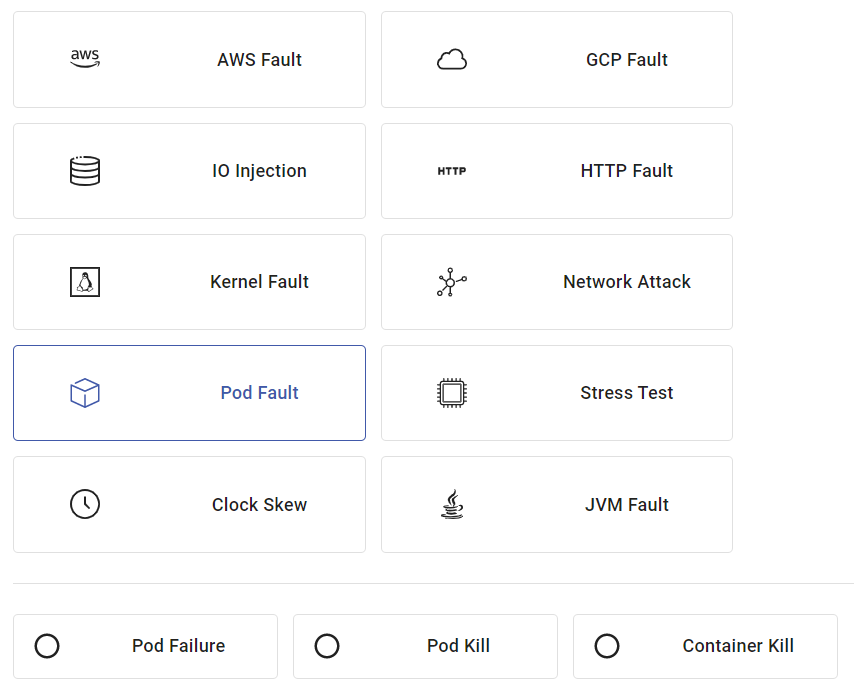
\includegraphics[scale=.7]{img/chaosmesh-experimenten.png}
    \caption{Chaos Mesh Experimenten per groep}
    \label{img:chaosmeshexperimenten}
\end{figure}

\subsubsection{Een eerste pod kill experiment opzetten via New Experiment} 

Het eerste experiment zal één willekeurige nginx pod uit de demo applicatie in namespace demoapp1 vernietigen. Volgende stappen omschrijven hoe men dit kan opzetten in het Chaos Dashboard: 
\begin{enumerate}
    \item Kies in de Dashboards pagina voor New Experiment. 
    \item In tabblad {\bf Experiment Type} kiest men bovenaan voor 'Kubernetes' en vervolgens in de lijst voor 'Pod Fault'. 
    \item Men krijgt als reactie op voorgaande keuze drie nieuwe keuzes te zien van experimenten die onder 'Pod Fault' beschikbaar zijn. Kies voor 'Pod Kill' en klik vervolgens op Submit om de keuze te bevestigen.
    \item In tabblad {\bf Experiment Info} configureert men vervolgens het experiment. Gebruik volgende configuraties om het Pod Kill experiment toe te passen op de nginx pods uit de demo applicatie:
        \begin{itemize}
            \item {\bf Scope}: Bij namespace stelt men in dat het PodChaos experiment in 'demoapp1' mag geplaatst worden.
            \item {\bf Metadata}: Geef zelf een naam aan het experiment.
            \item {\bf Label Selectors}: specifieer welke pods getroffen moeten worden o.b.v. de label, in dit geval 'app=nginx'.
            \item {\bf Mode}: Hier configureert men hoeveel pods getroffen moeten worden. Het experiment is gericht op één pod dus men kiest men 'Random One'. Alternatieve keuzes zijn een vast aantal, percentueel, allemaal ...
            \item {\bf Preview of Pods to be injected}: (Optioneel) Dit toont een lijst o.b.v. voorgaand gemaakte keuzes waarin men kan zien welke pods getroffen zullen worden door het experiment. Hier kan men eventueel nog pods de-selecteren die niet door het experiment getroffen mogen worden.
            \item Klik op Submit om de configuraties te bevestigen.
        \end{itemize}
    \item Wanneer zowel het Experiment Type als de Experiment Info via Submit bevestigd zijn zal nog een derde keer bevestigd moeten worden via Submit om het experiment daadwerkelijk te starten.
\end{enumerate}

\begin{figure}[h]
    \centering
    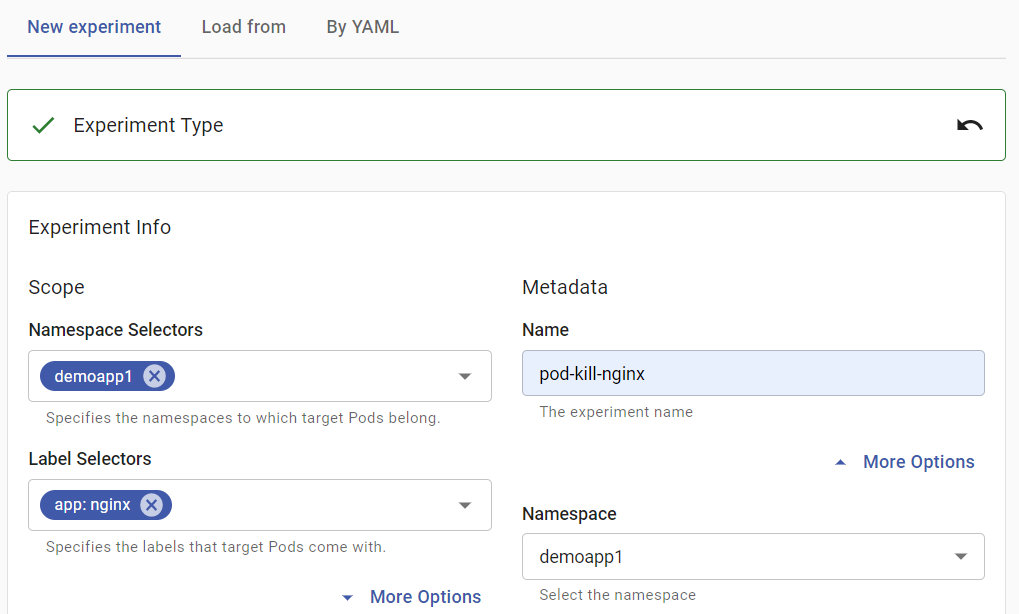
\includegraphics[scale=.7]{img/experiment-info.png}
    \caption{Configureren van experiment in Chaos Dashboard}
    \label{img:config-in-dashboard}
\end{figure}

Na de bevestiging ziet men het experiment verschijnen in het menu Experiments met als status 'Injecting'. Wanneer men hierop klikt zal extra info weergegeven worden waaronder de configuratie, de Events (die de fases van het experiment beschrijven) en de YAML-definitie van het experiment. 

Men kan een (statisch) overzicht van de pods opvragen in de Cloud Shell terminal m.b.v. commando {\bf kubectl get pods -n demoapp1}, maar nog een betere optie is om dit experiment op te volgen via k9s. Gebruik hiervoor het commando {\bf ./k9s -n demoapp1} om specifiek de pods in de namespace van de demo-applicatie te openen. Op deze manier kan men live volgen hoe na het bevestigen van het experiment één willekeurige nginx pod uit de demo-applicatie vernietigd wordt.
In de kolom 'Age' zal te zien zijn dat één van de nginx pods nog maar enkele seconden actief is. 

In bovenstaand stappenplan werd elke parameter van het experiment geconfigureerd in de GUI. In figuur \ref{img:config-in-dashboard} ziet men ook nog twee andere tabbladen nl.:
\begin{itemize}
    \item {\bf Load from:} bedoeld om configuratie van een alreeds uitgevoerd experiment te herladen en aan te passen. Let op: men moet de naam van het experiment wijzigen aangezien anders een foutmelding op het scherm zal verschijnen die zal aangeven dat het experiment alreeds bestaat.
    \item {\bf By YAML:} bedoeld om zelf een YAML-definitie te schrijven of een alreeds bestaande vanop het systeem in te laden.
\end{itemize} 

\subsubsection{Een experiment plannen via New schedule}

In vorige subsectie werd beschreven hoe een enkelvoudig experiment opgezet werd. Een meer praktische benadering van chaos engineering zou zijn om een experiment meerdere malen te herhalen om de applicatie op verschillende tijdstippen te testen. In het Chaos Dashboard kan men dit bekomen via de optie 'New schedule' in het Dashboard menu, of door direct naar het 'Schedules' menu te gaan. 

Op een gelijkaardige manier als voordien zal men het experiment kunnen configureren. Enkele extra parameters zullen hier ook geconfigureerd moeten worden nl.:
\begin{itemize}
    \item {\bf newS.basic.historyLimit:} het aantal logbestanden (records) er moeten bewaard worden.
    \item {\bf newS.basic.concurrencyPolicy:} toestaan dat het experiment gelijktijdig met andere experimenten wordt uitgevoerd.
    \item {\bf Schedule:} via een cron schedule aangeven op welke tijdstippen het experiment moet uitgevoerd worden. Een link naar de website \url{https://crontab.guru/} wordt meegegeven om deze parameter op een correcte manier te configureren.
\end{itemize}

Op een gelijkaardige manier als voordien zal nu een nieuw experiment opgezet worden genaamd 'kill-random-three' waarbij drie willekeurige pods in de demo applicatie vernietigd zullen worden elk uur op minuut 45. Deze keer zal geen gebruik gemaakt worden van een label dus zowel Apache als Nginx pods komen hierdoor in aanmerking.
De cron schedule die gebruikt wordt is 45 * * * *  (minuut / uur / dag / maand / dag v.d. week).

Geplande experimenten kunnen opgevolgd worden in het 'Schedules' menu. Hier zal men zien dat het experiment de status 'Running' krijgt. Deze status zal behouden worden tot wanneer men zelf beslist dit te stoppen door het experiment te archiveren. 

\subsubsection{Meerdere experimenten opzetten via New workflow}

Wanneer men meerdere experimenten wil uitvoeren in serie, parallel, in combinatie met een taak ... dan doet men dit d.m.v. een workflow te creëeren. In het Chaos Dashboard kan men dit bekomen via de optie 'New workflow' in het Dashboard menu, of door direct naar het 'Workflows' menu te gaan.

Een praktische benadering in een workflow zou zijn om parallel een experiment uit te voeren waarbij  willekeurige pods van een applicatie getroffen worden en ondertussen ook de bereikbaarheid van de applicatie herhaaldelijk te controleren gedurende de tijdspanne van het experiment. Dit zou men kunnen doen door een GET-request uit te sturen en te controleren als een HTTP-response met code 200 terugkeert, wat wil zeggen dat de request succesvol was. \autocite{MDN2022} 

Jammer genoeg is het opzetten van dit scenario in een workflow op het eerste zicht niet mogelijk. Men kan wel opteren voor één HTTP-request uit te sturen via de task type 'HTTP Request'. Na onderzoek bleek deze functionaliteit zich nog in een experimentele fase te bevinden. \autocite{ChaosMesh2022c}  
\newline Ook op de Chaos Mesh Q\&A pagina kan men lezen dat 'probe support' nog niet gepland staat om toegevoegd te worden aan de functionaliteiten van Chaos Mesh. \autocite{ChaosMesh2021}

Het iteratief herhalen van een experiment is wel mogelijk via een workflow, maar is vrij omslachtig. Men moet hierbij hetzelfde experiment meerdere malen configureren zodat dit achtereenvolgens uitgevoerd kan worden. Een voorbeeld van de YAML-definitie die ontstaan is bij het testen van het iteratief vernietigen van een willekeurige pod van de applicatie in namespace demoapp2 kan men in volgende link terugvinden: \href{https://github.com/KenBruggeman/BP_21-22/blob/master/bachelorproef/docs/chaosmesh-experimenten/iteration-test.yaml}{iteration-test.yaml}. \newline Een betere manier zou zijn om een iteratie als parameter mee te geven bij het opzetten van een enkelvoudig experiment. 

\subsection{Experimenten opzetten via de terminal}

Op de Chaos Mesh website vindt men heel wat voorbeeld YAML-definities van experimenten terug. Open volgende link naar de website en ga in het linkermenu naar 'Types of Chaos Experiments': \url{https://chaos-mesh.org/docs/}.

Hieronder krijgt men opnieuw de keuze tussen 'Kubernetes' en 'Physical Nodes' te zien. Als men verder gaat in optie Kubernetes ziet men dezelfde oplijsting als voordien in het Chaos Dashboard. In de documentatie van elk experiment ziet men o.a. hoe men via het Chaos Dashboard dit kan opzetten, maar ook een voorbeeld YAML-definitie die men via de terminal kan uitproberen.

\subsubsection{Experiment 1: pod-failure}

Een eerste experiment om via de terminal uit te proberen is het pod-failure experiment. Hierbij zal over een periode van dertig seconden één willekeurige pod van de PodTato-Head applicatie uit de namespace demoapp2 falen. 

Een alreeds aangepaste YAML-definitie van het hieronder beschreven pod-failure experiment kan men vinden via volgende link: \href{https://github.com/KenBruggeman/BP_21-22/blob/master/bachelorproef/docs/chaosmesh-experimenten/pod-failure.yaml}{pod-failure.yaml} 

Om manueel het pod-failure experiment te configureren gebruikt men volgend stappenplan. Hierbij wordt gebruik gemaakt van de voorbeeld YAML-definitie op de Chaos Mesh website.
\begin{enumerate}
    \item Ga op de Chaos Mesh website in het linkermenu naar Types of Chaos Experiments. Kies voor Kubernetes en vervolgens voor 'Simulate Pod Faults'.
    \item Kopieer de inhoud van de YAML-definitie in sectie 'pod-failure example'.
    \item Ga naar de Cloud Shell terminal en maak een nieuw bestand aan die `pod-failure.yaml` noemt in de directory 'chaosmesh-experiments'.
    \item Plaats de inhoud van het experiment in dit bestand en pas volgende zaken aan:
    \begin{itemize}
        \item wijzig de waarde bij parameter namespace (onder metadata) naar 'demoapp2'. 
        \item verwijder onder selector de parameter labelSelector en de toegewezen waarde.
        \item voeg onder selector een parameter 'namespaces' toe met de waarde 'demoapp2'. Als voorbeeld kan men kijken naar de configuratie van het pod-kill.yaml bestand verderop in de documentatie.
        \end{itemize} 
    \item Sla de wijzigingen op.
    \item Voer het experiment uit via commando {\bf kubectl apply -f pod-failure.yaml}. Men zal hierbij volgende melding te zien krijgen: 'podchaos.chaos-mesh.org/pod-failure-example created' 
\end{enumerate}

Nota: Indien men hier de foutmelding 'Admission webhook "vauth.kb.io" denied the request' te zien krijgt kan men een workaround toepassen via volgend commando uit te voeren en nadien het experiment te herhalen:\newline {\bf kubectl delete validatingwebhookconfigurations.admissionregistration.k8s.io validate-auth} \autocite{Keao2021} 
  
Men kan bij het uitvoeren van het pod-failure experiment zien via k9s dat een restart afgedwongen wordt bij één van de pods in de Podtato-Head applicatie. Wanneer men via k9s op de getroffen pod staat kan men de beschrijving openen door op 'D' te duwen. Onderaan deze pagina in sectie Events zal men zien hoe de pod gedwongen wordt om te herstarten doordat de definitie van de container gewijzigd is door de foutinjectie.

\begin{figure}[h]
    \centering
    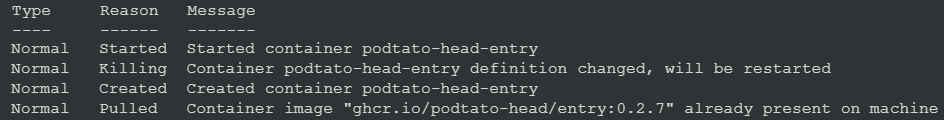
\includegraphics[scale=.7]{img/k9s-pod-described.png}
    \caption{opvragen van Events van getroffen pod via k9s}
\end{figure}

Het starten van het pod-failure experiment creëerde een 'podchaos' object in de demoapp2 namespace. Dit kan men controleren via commando {\bf kubectl get podchaos -n demoapp2}. Indien men Events wil opvragen van het bovenstaand experiment dan spreekt men het 'podchaos' object aan via commando {\bf kubectl describe podchaos pod-failure-example -n demoapp2}.

Nota: Afhankelijk van het type experiment zal dit object variëren vb. bij een later experiment waarbij CPU-belasting zal opgewekt worden noemt dit object 'stresschaos'. Deze info kan men afleiden uit de parameter 'kind' in de YAML-definitie van het experiment. 

Men zal eveneens zien dat dit experiment toegevoegd is in het Experiments menu van het Chaos Dashboard.

\subsubsection{Een experiment herhalen via de terminal}

Wanneer men het pod-failure experiment zou willen herhalen in de terminal, dan is dit niet mogelijk door gewoon opnieuw het {\bf kubectl apply -f pod-failure.yaml} commando uit te voeren. Dit zal namelijk volgende melding genereren: 'podchaos.chaos-mesh.org/pod-failure-example unchanged'. 

Men moet steeds eerst het bestaande podchaos object verwijderen via commando {\bf kubectl delete podchaos pod-failure-example -n demoapp2} alvorens een experiment opnieuw te kunnen uitvoeren. 

\subsubsection{Experiment 2: NetworkChaos experiment}

In dit experiment zal gedurende zestig seconden een communicatiestoring uitgelokt worden tussen de Apache en Nginx pods van de demo-applicatie in namespace demoapp1. Vooraf kan men al testen als de communicatie tussen beiden succesvol is. Dit doen men op volgende manier: 
\begin{lstlisting}
# Bewaar eerste Apache pod in environment variabele
$ pod=$(kubectl get pods -n demoapp1 -l app=apache \
 -o jsonpath='{.items[0].metadata.name}')

# Open een shell in de container binnenin de Apache POD
# en controleer als nginx pods bereikt kunnen worden
$ kubectl exec $pod -n demoapp1 -it -- /bin/sh \
 -c "curl nginx"
 
# Bewaar eerste Nginx pod in environment variabele
$ pod2=$(kubectl get pods -n demoapp1 -l app=nginx \
-o jsonpath='{.items[0].metadata.name}')

# Open een shell in de container binnenin de Nginx POD
# en controleer als Apache pods bereikt kunnen worden
$ kubectl exec $pod2 -n demoapp1 -it -- /bin/sh \
-c "curl apache"
\end{lstlisting}

Beide controles tonen de output van de Apache of Nginx website waardoor bevestigd is dat de communicatie tussen deze pods/services correct verloopt. 

Het toepassen van dit experiment verloopt opnieuw door de YAML-definitie van de officiële Chaos Mesh website te raadplegen en dit op het systeem over te brengen in een nieuw bestand genaamd 'network-partition.yaml'.
\newline Men kan alreeds een voorgedefinieerde YAML-definitie van dit NetworkChaos experiment via volgende link terugvinden: \href{https://github.com/KenBruggeman/BP_21-22/blob/master/bachelorproef/docs/chaosmesh-experimenten/network-partition.yaml}{network-partition.yaml}

Voer het experiment vervolgens uit via {\bf kubectl apply -f network-partition.yaml}. 

Door nu opnieuw de commando's toe te passen waarmee men de bereikbaarheid van de nginx en Apache pods kon testen zal men nu gedurende de duurtijd van het experiment geen output meer te zien krijgen. 

Nota: Later bij het documenteren en herproberen van alle experimenten mislukte het NetworkChaos experiment met de melding 'Failed to apply chaos: PodNetworkChaos.chaos-mesh.org is invalid: spec.ipsets.cidrs: Required value'. \newline Een reden hiervoor kon echter niet gevonden worden en bij online troubleshooting kon deze foutmelding geen enkele concrete oplossing tonen.  

\subsubsection{Experiment 3: Stresschaos experiment}

In dit experiment zal over een periode van twee minuten een belasting van ongeveer 200 MB geheugenverbruik gegenereerd worden op de nginx pods in de demo-applicatie in namespace demoapp1. Vervolgens zal het nut aangetoond worden van het Kubernetes object {\bf HorizontalPodAutoscaler (HPA)}, die extra pods zal creëeren wanneer een geconfigureerde CPU- of geheugenlimiet overschreden wordt.

Bij de demo-applicatie in demoapp1 is een kanttekening te maken aangezien deze oorspronkelijk opgezet is zonder een limiet op de resources die het mag gebruiken. Hierdoor zou een applicatie alle resources van een node kunnen aanspreken, maar dit is geen ideaal scenario. Zo is een pod ingesteld volgens 3 QoS klasses. Pods zonder geconfigureerde resource management vallen onder de klasse 'best effort' en komen hierdoor als eerste in aanmerking om vernietigd te worden wanneer de node resources beperkt worden. \autocite{Tatiyana2020}

Om de pods in de demoapp1 namespace te configureren zodanig deze maximum 200 mCPU en 256MB gebruiken voert men volgende twee commando's uit \autocite{Kubernetes2022c}: 
\begin{lstlisting}
    $ kubectl set resources deployment nginx -n demoapp1 \
    --limits=cpu=200m,memory=256Mi
    
    $ kubectl set resources deployment apache -n demoapp1 \
    --limits=cpu=200m,memory=256Mi
\end{lstlisting}

De officiële documentatie voor een StressChaos experiment op te zetten kan men hier terugvinden: \url{https://chaos-mesh.org/docs/simulate-heavy-stress-on-kubernetes/}

Men kan ook gebruik maken van de alreeds geconfigureerde YAML-definitie voor dit specifieke experiment via volgende link: \href{https://github.com/KenBruggeman/BP_21-22/blob/master/bachelorproef/docs/chaosmesh-experimenten/memory-stress.yaml}{Experiment 3: memory-stress.yaml}

Maak een nieuw bestand aan genaamd 'memory-stress.yaml' in de directory chaosmesh-experiments en plaats de inhoud hierin. Start vervolgens het experiment op via commando {\bf kubectl apply -f memory-stress.yaml}

Tijdens de uitvoer van het experiment kan men via het Google Cloud Platform de geheugenbelasting van de nginx pods opvolgen. Open het dropdownmenu in de linkerbovenhoek en kies in deze lijst {\bf Kubernetes Engine} en vervolgens {\bf Workloads} om naar de pods in de demoapp1 namespace te gaan. Wanneer men hier op nginx klikt zal een overzicht geopend worden waarin drie metrics opgevolgd worden nl. CPU, geheugen en diskverbruik.

Optioneel: Men kan bij elk van deze metrics in de rechterbovenhoek het menu openen en verder gaan naar de {\bf Metrics Explorer}.

\begin{figure}[h]
    \centering
    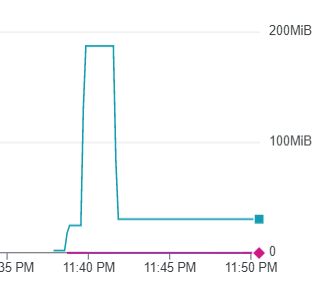
\includegraphics{img/nginx-memorystress.png}
    \caption{GKE workloads: belasten van geheugen nginx pods}
\end{figure}

\subsubsection{Kubernetes object: HorizontalPodAutoscaler}
\label{subsec: HPA}
Wanneer pods zwaar belast worden qua geheugen (of CPU) dan zal dit een negatieve impact hebben op de goede werking van een applicatie. Een te zware belasting waarbij een pod meer resources verbruikt dan toegelaten zal zelf resulteren in het beëindigen van de pod door de kernel Out-Of-Memory killer (OOMkill). Dit proces zal Kubernetes helpen om het geheugen te beheren wanneer pods aan nodes toegewezen worden en zal eveneens beslissingen nemen welke pods te vernietigen wanneer resources op de node in gevaar komen. \autocite{Alletto2021} 

Een antwoord bieden om dit risico te helpen vermijden is het gebruiken van het Kubernetes object {\bf HorizontalPodAutoscaler}. Dit object zal ervoor zorgen dat extra pods gegenereerd worden wanneer een geconfigureerde resources threshold overschreden wordt.

Een voorgeconfigureerde YAML-definitie voor het creëeren van een HPA kan men hier terugvinden: 
\href{https://github.com/KenBruggeman/BP_21-22/blob/master/bachelorproef/docs/chaosmesh-experimenten/hpa.yaml}{HorizontalPodAutoscaler definitie: hpa.yaml} 

Creëer een nieuwe YAML-definitie op het systeem genaamd 'hpa.yaml' en voer dit vervolgens uit via commando {\bf kubectl apply -f hpa.yaml}. 

Men kan nu niet zomaar het experiment herhalen maar zal eerst het bestaande experiment moeten verwijderen. Dit doet men via commando {\bf kubectl delete stresschaos memory-stress-example -n demoapp1}. Nu kan men opnieuw de YAML-definitie van het experiment oproepen via commando {\bf kubectl apply -f memory-stress.yaml}. Via k9s kan men vervolgens opvolgen hoe drie extra pods aangemaakt worden tijdens de belasting van het geheugen.
 
\subsection{Conclusie Chaos Mesh}

De installatie van Chaos Mesh verloopt snel en eenvoudig, zowel met het onliner script in een lokale omgeving als via de package manager Helm in de cloud omgeving. Het opzetten van het Chaos Dashboard daarentegen ging enkele keren mis waardoor dit onbruikbaar was. Controle in de browser via de Developer Tools (F12) gaven hierbij een resem fouten aan. Pas na enkele pogingen kon een correcte werking bekomen worden, maar de oorzaak waardoor het in de eerste plaats fout ging is nooit achterhaald.

Het Chaos Dashboard is gebruiksvriendelijk opgesteld en vereist weinig kennis om direct aan de slag te kunnen. Experimenten opzetten is eenvoudig, maar de extra functionaliteit tijdens de uitvoer van een experiment ontbreekt jammer genoeg. Zo is het bv. niet mogelijk om een experiment op te zetten waarbij doorlopende controle van de bereikbaarheid van een applicatie getest wordt, kan men geen logs raadplegen van uitgevoerde experimenten ... Ook zou het praktisch zijn om in de configuratie van een experiment aan te geven dat dit iteratief uitgevoerd dient te worden bv. elke twintig seconden herhalen gedurende een periode van vijf minuten. Dit kan men enkel bekomen door een workflow te configureren waarbij enkelvoudige experimenten in serie herhaald worden, maar dit is vrij omslachtig aangezien telkens dezelfde configuratie gewoonweg herhaald wordt.

Experimenten opzetten via de terminal is mogelijk, maar biedt geen meerwaarde t.o.v. het uitvoeren van experimenten via het Chaos Dashboard. Meeste experimenten in Chaos Mesh werden wel toegepast in de terminal doordat het Chaos Dashboard bij eerdere installaties onbruikbaar was. Het is ook jammer dat een experiment niet gewoon kan herhaald worden zonder dat eerst het origineel gewist moet worden. Er kwamen ook enkele foutmeldingen bij het opzetten en uitvoeren van de experimenten via de terminal die moeilijk te troubleshooten waren door een gebrek aan documentatie.  
 
\section{Litmus}

In de zoektocht naar een chaos engineering tool die net zoals voorgaande tool ChaosMesh zowel experimenten kon uitvoeren vanuit de terminal als via de browser, werd de keuze gemaakt om Litmus te onderzoeken. 

Het Litmus project startte in 2017 met als doel om simpele chaos experimenten op te zetten in een Kubernetes cluster. Het werd een Cloud Native Computing Foundation (CNCF) sandbox project in 2020, en wordt vandaag onderhouden door vijf verschillende organisaties. Sinds begin 2022 is het project geëvolueerd naar een CNCF incubating project. \autocite{CNCF2022}

\subsection {Vereisten}
\label{sec:litmusvereisten}

Om Litmus te kunnen installeren moeten drie zaken aanwezig zijn \autocite{Litmus2022}: 
\begin{itemize}
    \item Kubernetes versie 1.17 of recenter
    \item Een Persistent Volume van 1GB waar Litmus de chaos configuratie en chaos-metrics zal opslaan. Standaard zal Litmus gebruik maken van de default storage class om deze Persistent Volume toe te wijzen.
    \item Helm versie 3 of kubectl 
\end{itemize}

De installatie van Litmus is enkel toegepast in GKE waar een default storage class aanwezig is. Dit is echter niet het geval bij de lokale clusters eerder opgezet via Kubeadm en Kubespray. Verder onderzoek als deze tool kan geïnstalleerd worden in een lokale omgeving is hierdoor nog vereist. 

\subsection{Installatie}

De installatie van Litmus verloopt in volgend beschreven stappenplan via Helm. Alternatief kan men ook de installatieprocedure via de kubectl commandline tool uitvoeren. Raadpleeg hiervoor de bron in \ref{sec:litmusvereisten}.   

De installatie kan men opsplitsen in twee delen. Eerst zullen de benodigde pods geïnstalleerd worden om Litmus op het systeem te krijgen. Nadien zal via de browser de toegang geconfigureerd worden tot het Litmus ChaosCenter, vanwaar men later eveneens experimenten zal kunnen uitvoeren. 

Voer volgende stappen uit om Litmus op het systeem te installeren:
\begin{lstlisting}[language=bash]
# Voeg de Litmus helm repository toe 
$ helm repo add litmuschaos https://litmuschaos.github.io/litmus-helm/

# Optioneel: controleer als repo toegevoegd is op het systeem
$ helm repo list

# Maak een namespace aan waaronder Litmus toegevoegd wordt
$ kubectl create ns litmus

# Installeer Litmus in de namespace litmus
$ helm install chaos litmuschaos/litmus --namespace=litmus

# Optioneel: verifieer de installatie
# Pods frontend, database (mongo) en server zouden aanwezig moeten zijn.
$ kubectl get pods -n litmus
\end{lstlisting}

\subsubsection{Firewall regels configureren}

Vooraleer men via de browser connectie kan maken met het Litmus ChaosCenter zullen eerst de nodige firewall regels moeten geconfigureerd worden. Om te weten te komen welke poorten open gezet moeten worden voert men commando {\bf kubectl get svc -n litmus} uit. \newline Dit toont alle actieve services in de litmus namespace. Daar ziet men o.a. dat voor de eerder vernoemde frontend- en server pod een Nodeport service is geconfigureerd. Deze laten toe om de pod van buitenaf te betreden. 

Voer o.b.v. info uit de output van vorig commando volgende stappen uit om de firewall te configureren. Hierbij is vooral het poortnummer in kolom Ports van belang. Deze poorten variëren echter bij elke installatie. Volgende commando's configureren firewall regels specifiek voor een GKE cluster en kunnen dus niet gebruikt worden in een lokale omgeving. Verder onderzoek hoe deze poorten te openen in een lokale omgeving is hierdoor nog nodig.  
\begin{lstlisting}[language=bash]
# Firewall regel die verkeer op poort frontend service toelaat.
# Gebruik frontend service poortnummer (na de dubbelpunt) 
$ gcloud compute firewall-rules create frontend-service-rule \
 --allow tcp:[port]

# Firewall regel die verkeer op poort server service toelaat. 
# Gebruik één v.d. server service poortnummers (na de dubbelpunt) 
$ gcloud compute firewall-rules create server-service-rule \
--allow tcp:[port]
\end{lstlisting}

Bij elk van bovenstaande commando's zal men bij een succesvolle uitvoer de regels 'Creating firewall...working..Created' en 'Creating firewall...done' te zien krijgen. 

\subsubsection{Toegang configureren tot Litmus ChaosCenter}
\label{subsec:chaoscenter}

Om via de browser naar het Litmus ChaosCenter te gaan kan men gebruik maken van één van de externe IP-adressen van de nodes. Deze kan men bekomen door in de terminal het commando {\bf kubectl get nodes -o wide} uit te voeren. Ook zal men het poortnummer nodig hebben van de frontend service, waar eerder een firewall regel voor geconfigureerd is. Gebruik {\bf http://[node IP-adres]:[frontend service poort]} in de browser om toegang te krijgen tot Litmus ChaosCenter. 

Wanneer men voor het eerst connecteert met het Litmus ChaosCenter kan men gebruik maken van de hieronder vermelde default credentials. Vervolgens zal men direct een nieuw wachtwoord moeten configureren alvorens de toegang te verkrijgen tot het Litmus ChaosCenter.
\begin{itemize}
    \item user = admin
    \item wachtwoord = litmus
\end{itemize}

\begin{figure}[h]
    \centering
    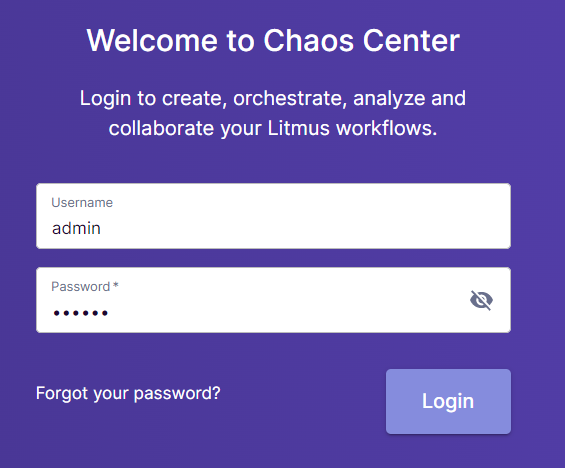
\includegraphics[scale=.5]{img/chaoscenter-login.png}
    \caption{login Litmus ChaosCenter}
\end{figure}

Later in dit onderzoek, vanaf hoofdstuk \ref{subsec:expchaoscenter}, zal omschreven worden hoe een experiment op te zetten via deze GUI. 
 
Nu de accountactivatie in Litmus ChaosCenter afgerond is zal men heel wat extra pods terugvinden in de namespace litmus. Dit kan men controleren door in de terminal het commando {\bf kubectl get pods -n litmus} uit te voeren. Een eerder gecreëerde cluster waarbij de resources per node te beperkt waren zorgde hier echter voor een falende pod genaamd 'event-tracker-[...]'. Deze pod bleef de status Pending behouden en door de pod te beschrijven via commando {\bf kubectl describe pod event-tracker-[...] -n litmus} kon onderaan bij Events te zien zijn dat onvoldoende CPU de oorzaak was. (zie onderstaande output)
 
\begin{lstlisting}[language=bash]
-- voorgaande output weggelaten --
-- volgende output ingekort     --
Events:
Type     Reason       From        Message
----     ------       ----        -------
Warning  Failed...    scheduler   0/3 nodes are available
                                  : 3 Insufficient cpu.
\end{lstlisting}
 
Vandaar bij voorgaand hoofdstuk in sectie \ref {sec:cloudclustersetup} het nodige belang gehecht werd aan voldoende resources toe te wijzen aan de nodes in de cluster. Volgende output toont aan dat de autoscaling configureren zijn nut bewees bij het herinstalleren van Litmus: 

\begin{lstlisting}[language=bash]
-- voorgaande output weggelaten --
-- volgende output ingekort     --
Events:
Type     Reason        From        Message
----     ------        ----        -------
Warning  Failed...     scheduler   0/3 nodes are available: 
                                   3 Insufficient cpu
Normal   Scheduled     scheduler   Successfully assigned ... 
Normal   Triggered...  autoscaler  pod triggered scale-up: 
                                   3 -> 4 (max: 6)
\end{lstlisting}

\subsection{Litmus experimenten uitvoeren via de terminal}

Vooraleer men experimenten kan uitvoeren moet men eerst volgende Litmus concepten begrijpen:
\begin{itemize}
    \item {\bf Chaos Experiment:} De generieke low-level code van een experiment waar men niks hoeft in te wijzigen.
    \item {\bf Chaos Engine:} De parameters waarmee men een experiment specifiek gaat richten naar een bepaalde applicatie/pod/... m.a.w. de connectie tussen applicatie en ChaosExperiment die men via een YAML-definitie configureert.
    \item {\bf Chaos Result:} Het resultaat van de uitvoer van een experiment. 
\end{itemize} 
 
Eerst zal in volgende subsecties een theoretische benadering geformuleerd worden hoe men een experiment dient op te zetten om uitgevoerd te worden via de terminal. Nadien wordt beschreven hoe het eerste experiment pod-delete opgezet kan worden. Vervolgens kan men nog een aantal andere uitgevoerde experimenten via de terminal terugvinden, alvorens over te gaan tot het uitvoeren van experimenten via de browser m.b.v. Litmus ChaosCenter.
 
\subsubsection{Experimenten installeren op het systeem}
\label{subsec:experimenteninstalleren}

Een experiment uit bovenstaande concept Chaos Experiment wordt bewaard in de Litmus Chaos Hub.  
Alle mogelijke Litmus experimenten kan men hier terugvinden, geklasseerd in verschillende categorieën. \autocite{ChaosHub2022} 

Men dient eerst de nodige categorie van experimenten te installeren in dezelfde namespace(s) van de demo-applicatie(s). De experimenten die via de terminal uitgevoerd worden vallen allen onder categorie {\bf generic/all-experiments}. \newline Om deze experimenten te installeren voert men volgend commando uit voor zowel de namespaces demoapp1 en demoapp2:
\begin{lstlisting}[language=bash]
$ kubectl apply -f \
https://hub.litmuschaos.io/api/chaos/2.7.0?file=charts/generic\
/experiments.yaml -n demoapp[1 en 2]
\end{lstlisting}

\subsubsection{Permissies van een experiment instellen}

Het uitvoeren van deze experimenten moet eerst voorafgegaan worden door de nodige permissies te configureren via {\bf Role Based Access Control (RBAC)}. Hierdoor verkrijgt het later beschreven experiment in de ChaosEngine de toestemming om uitgevoerd te worden binnen een bepaalde namespace. Permissies configureert men bij elk experiment wanneer men dit via de terminal uitvoert. 

Een vooraf gedefinieerde RBAC-configuratie per experiment kan men terugvinden via volgende link: \url{https://litmuschaos.github.io/litmus/experiments/categories/contents/}

De YAML-definitie in sectie {\bf Minimal RBAC configuration} slaat men op in een bestand onder een nieuw gecreëerde subdirectory (bv. serviceaccounts) in de alreeds bestaande directory litmus-experiments. Men hoeft enkel nog de waarde van elke parameter 'namespace' in dit bestand aanpassen naar de naam van de namespace waarin het experiment uitgevoerd wordt m.a.w. de namespace demoapp1 of demoapp2. \newline Via commando {\bf kubectl apply -f [bestand].yaml} maakt men vervolgens de nodige bestanden aan om de permissies te activeren.  

\subsubsection{Een ChaosEngine definiëren}

Nu de nodige permissies ingesteld zijn kan men een ChaosEngine definiëren waarin de link wordt gelegd naar het ChaosExperiment. Ook deze definitie kan men terugvinden in eerder vermelde link, in de sectie {\bf Experiment Examples}. Kopieer ook hier de inhoud en sla deze op in een nieuw bestand in de directory litmus-experiments. \autocite{Experiments2022}. 

Men zal zien dat in de ChaosEngine definitie de ServiceAccount aangesproken wordt. De parameter jobCleanUpPolicy zal er voor zorgen dat de 'helper pods' die Litmus lanceert tijdens het experiment terug verwijderd zullen worden na afloop.

Alle mogelijke parameters in aanvulling van een experiment kan men terugvinden in de sectie {\bf Experiment tunables}. Zo kan men o.a. beslissen via parameter CHAOS\textunderscore INTERVAL een experiment in iteraties uit te voeren, via parameter PODS\textunderscore AFFECTED\textunderscore PERC het percentage getroffen pods in te stellen ... 

\subsubsection{Een experiment uitvoeren}
\label{subsec:experimentuitvoeren}
Vervolgens is men klaar om een experiment uit te voeren. Dit kan men doen via commando {\bf kubectl apply -f [experiment-naam].yaml}. Dit commando zal géén output genereren. 

Tijdens de uitvoer kan men via de UI monitoring tool k9s het experiment live opvolgen. Hierin zal men eveneens zien dat in de demoapp[1/2] namespace tijdelijke helper pods gelanceerd worden om de uitvoer van het experiment te faciliteren. 

Enkele handige commando's om de uitvoer tijdens-, of het resultaat na een experiment te controleren zijn:
\begin{lstlisting}[language=bash]
# ChaosEngine object(en) oplijsten
$ kubectl get chaosengine -n demoapp[1 of 2]

# Het verloop van experiment tonen door het 
# ChaosEngine object te beschrijven
$ kubectl describe chaosengine [chaosengine] -n demoapp[1 of 2]

# ChaosResult object(en) oplijsten
$ kubectl get chaosresult -n demoapp[1/2]

# Het resultaat van experiment tonen door het 
# ChaosResult object te beschrijven
$ kubectl describe chaosresult [chaosresult] -n demoapp[1 of 2]
\end{lstlisting}

\subsection{Experiment 1: Nginx pod delete}

Bovenstaande theoretische benadering hoe men m.b.v. Litmus een experiment kan opzetten via de terminal zal in dit hoofdstuk omgezet worden naar de praktijk. De ChaosEngine van dit experiment, inclusief volgende experimenten kan men eveneens raadplegen via volgende link naar Git repository: \url{https://github.com/KenBruggeman/BP\textunderscore 21-22/blob/master/bachelorproef/docs/litmus%20experimenten/}

Het eerste experiment die aan bod komt is het vernietigen van een Nginx pod in de namespace demoapp1. In deze namespace is ook een Deployment met Apache pods actief, die gevrijwaard zal blijven van de impact van dit experiment door dit zorgvuldig te configureren in de ChaosEngine definitie. 

Nota: Experiment 2 en 3 zijn uitbreidingen op dit experiment en zullen dus gebruik maken van de alreeds geconfigureerde permissies onder subdirectory litmus-experiments/serviceaccounts/ van experiment 1. Dit kan men eveneens zien in de ChaosEngine definitie, waar de naam onder parameter 'experiments' steeds pod-delete zal zijn. 

De bedoeling van dit experiment is aantonen dat een pod vernietigen in Kubernetes opgevangen wordt door de ReplicaSet die bij een Deployment hoort. Deze zal er steeds voor zorgen dat het gewenste aantal pods van een Deployment verzekerd wordt. Bij creatie van de Nginx Deployment in demoapp1 werd in het commando aangegeven dat drie replicas moesten bestaan. Dit experiment zal slechts 1 willekeurige Nginx pod vernietigen.  

De nodige experimenten, geïnstalleerd in \ref{subsec:experimenteninstalleren} zijn alreeds aanwezig zowel in de namespace demoapp1 als demoapp2.
  
Via volgend stappenplan stelt men de permissies van het eerste pod-delete experiment en creëert men een ChaosEngine waarmee het experiment kan uitgevoerd worden: 
\begin{enumerate}
    \item Open volgende link via de browser: \url{https://litmuschaos.github.io/litmus/experiments/categories/contents/} 
    \item Ga in het linkermenu via de dropdownlist Kubernetes - Generic - Pod Chaos naar het experiment {\bf Pod Delete}. Daar vindt men de beschrijving en configuratie van dit experiment.
    \item Kopieer de YAML-definitie in sectie {\bf Minimal RBAC configuration}
    \item Ga via de Cloud Shell terminal naar de subdirectory /litmus-experiments/servicaccounts/
    \item Maak een nieuwe file pod-delete-sa.yaml aan en kleef de inhoud uit voorgaande stap hierin
    \item Verander bij elke parameter 'namespace:' de waarde default naar demoapp1, en sla vervolgens op.
    \item Voer het bestand uit via commando {\bf kubectl apply -f pod-delete-sa.yaml}. Dit zal volgende output genereren:
\begin{lstlisting}[language=bash]    
serviceaccount/pod-delete-sa created
role.rbac.authorization.k8s.io/pod-delete-sa created
rolebinding.rbac.authorization.k8s.io/pod-delete-sa created
\end{lstlisting}
    \item Herhaal bovenstaande stappen 1 en 2. Ga naar sectie {\bf Experiment Examples} en kopieer de inhoud van dit bestand.
    \item Maak een YAML-bestand aan in de directory litmus-experiments en noem dit bv. nginx-pod-kill.yaml
    \item Kleef de inhoud uit sectie {\bf Experiment Examples} in dit YAML-bestand en wijzig  de waarde van parameters namespace naar demoapp1, en applabel naar app=nginx, zodat het experiment specifiek gericht wordt op de nginx pods van de demo-applicatie in namespace demoapp1.
    \item Sla het bestand op en voer het experiment uit via {\bf kubectl apply -f nginx-pod-kill.yaml}
    \item Volg het experiment op via k9s of via commando's uit subsectie \ref{subsec:experimentuitvoeren}: Een experiment uitvoeren.
\end{enumerate}

Dit experiment toonde de werking van de ReplicaSet die binnen enkele seconden na het vernietigen van een willekeurige Nginx pod alreeds een nieuwe pod heeft gecreëerd.

\subsection{Experiment 2: Nginx pod delete met iteratie}

Link naar het Git repository bestand ChaosEngine-definitie \href{https://github.com/KenBruggeman/BP_21-22/blob/master/bachelorproef/docs/litmus%20experimenten/nginx-pod-kill.yaml}{Experiment 2: nginx-pod-kill.yaml}

In dit experiment wordt een parameter toegevoegd aan de bestaande ChaosEngine uit voorgaand experiment die ervoor zorgt dat de uitvoer elke tien seconden herhaald zal worden. 

Open het YAML-bestand nginx-pod-kill.yaml, ga naar sectie 'env' en verleng de tijd van het experiment naar zestig seconden. Voeg eveneens een extra parameter 'CHAOS\textunderscore INTERVAL' toe om de iteratie in te stellen. Zie onderstaand vb.:
\begin{lstlisting}
- name: TOTAL_CHAOS_DURATION
  value: '60'
- name: CHAOS_INTERVAL
  value: '10'
\end{lstlisting}

Sla vervolgens op en start het experiment op dezelfde manier als voordien via {\bf kubectl apply -f nginx-pod-kill.yaml}. 

Men kan bij de uitvoer van het experiment zien via k9s dat elke tien seconden één willekeurige pod vernietigd wordt gedurende één minuut waardoor de ReplicaSet meermaals getriggerd zal worden om een nieuwe pod te creëeren.

Om te zien als dit een impact heeft op de bereikbaarheid van de Nginx pods zal in volgend experiment een http-probe toegevoegd worden aan de ChaosEngine definitie. 

\subsection{Experiment 3: Nginx pod delete met iteratie en probe}

Link naar het Git repository bestand ChaosEngine-definitie \href{https://github.com/KenBruggeman/BP\textunderscore 21-22/blob/master/bachelorproef/docs/litmus%20experimenten/nginx-pod-kill-probed.yaml}{Experiment  3: nginx-pod-kill-probed.yaml}

In dit experiment controleert men via een {\bf http-probe} als de applicatie bereikbaar is gedurende de uitvoer van het experiment. Via een http-probe wordt een GET-request gestuurd naar een opgegeven IP-adres, in dit geval het extern IP-adres van de LoadBalancer (of NodePort) service van de Nginx pods. Door eveneens een HTTP-response code op te geven die men verwacht terug te krijgen zal kunnen gecontroleerd worden als de applicatie tijdig bereikbaar is. 

Er zijn vier verschillende probes beschikbaar in Litmus, waarvan men een vooraf geconfigureerde YAML-definitie kan terugvinden en toepassen in een ChaosEngine. Deze vindt men hier terug: \url{https://docs.litmuschaos.io/docs/concepts/probes/} 

Men kan een http-probe configureren via verschillende parameters die o.a. bepalen:
\begin{itemize}
    \item hoe snel men de response verwacht
    \item hoeveel keer deze probe moet uitgevoerd worden
    \item hoeveel keer opnieuw mag geprobeerd worden wanneer de probe faalt
    \item ...
\end{itemize}
    
Kopieer de inhoud van dit bestand en sla dit lokaal op via de Cloud Shell terminal in een nieuw YAML-bestand genaamd nginx-pod-kill-probed.yaml. Voer het experiment vervolgens uit via commando {\bf kubectl apply -f nginx-pod-kill-probed.yaml} en volg opnieuw op via k9s. 

Men kan de status van de http-probe nadien controleren door het resultaat van het experiment op te vragen die bewaard wordt in een ChaosResult object. Om de exacte naam van dit object te weten te komen gebruikt men commando {\bf kubectl get chaosresults -n appdemo1}. \newline Eens men de naam kent kan via commando {\bf kubectl describe chaosresult [chaosresult-naam] -n appdemo1} het resultaat opgevraagd worden.

Een deel van de output, waarin aangetoond wordt dat de probe geslaagd is en de nginx website nog bereikbaar is wanneer nginx pods vernietigd worden, kan men hieronder zien: 
\begin{lstlisting}
--vorige output weggelaten--    
Probe Status:
    Name:  check-frontend-access-url
    Status:
        Continuous:  Passed 👍   
    Type:          httpProbe
\end{lstlisting}

Dit experiment is handig om de responsetijd van een website te controleren wanneer deze te kampen krijgt met pods die plots vernietigd worden. 

(Optioneel) Door onderaan in de ChaosEngine-definitie bij sectie 'env' de parameter 'PODS\textunderscore AFFECTED\textunderscore PERC' toe te voegen kan men een hoger percentage instellen van pods die getroffen worden door het experiment.

\subsection{Experiment 4: Geheugen belasten van nginx pods}

In dit experiment zal het geheugen belast worden van de nginx pods in de demo-applicatie in namespace demoapp1. Applicaties in een productieomgeving kunnen te maken krijgen met pieken in resourcegebruik, dit door verwachte maar eveneens onverwachte redenen. Vandaar het belangrijk is te testen hoe een applicatie reageert in deze omstandigheden, en welke manieren er in Kubernetes bestaan om hulp te bieden in zulke situaties. 

Bij de demo-applicatie in demoapp1 is een kanttekening te maken aangezien deze oorspronkelijk opgezet is zonder een limiet op de resources die het mag gebruiken. Hierdoor zou een applicatie alle resources van een node kunnen aanspreken, maar dit is geen ideaal scenario. Zo is een pod ingesteld volgens 3 QoS klasses. Pods zonder geconfigureerde resource management vallen onder de klasse 'best effort' en komen hierdoor als eerste in aanmerking om vernietigd te worden wanneer de node resources beperkt worden. \autocite{Tatiyana2020}

Om de pods in de demoapp1 namespace te configureren zodanig deze maximum 200 mCPU en 256MB gebruiken voert men volgende twee commando's uit \autocite{Kubernetes2022c}: 
\begin{lstlisting}
$ kubectl set resources deployment nginx -n demoapp1 \
--limits=cpu=200m,memory=256Mi

$ kubectl set resources deployment apache -n demoapp1 \
--limits=cpu=200m,memory=256Mi
\end{lstlisting}

Link naar het Git repository bestand ChaosEngine-definitie \href{https://github.com/KenBruggeman/BP_21-22/blob/master/bachelorproef/docs/litmus%20experimenten/nginx-pod-memory-hog.yaml}{Experiment 4: nginx-pod-memory-hog.yaml}

Men kan de inhoud uit bovenstaande link kopiëren en plaatsen in een nieuwe ChaosEngine in directory litmus-experiments met als naam 'nginx-pod-memory-hog.yaml'.

Dit experiment zal een nieuwe RBAC-configuratie vereisen, aangezien een ander ChaosExperiment nl. 'pod-memory-hog' wordt aangeroepen in de ChaosEngine. Alle benodigde configuratie kan men raadplegen via volgende link:
\url{https://litmuschaos.github.io/litmus/experiments/categories/pods/pod-memory-hog/}

Men kan op een identieke manier zoals bij experiment 1 te werk gaan door een bestand 'pod-memory-hog-sa.yaml' in de subdirectory /litmus-experiments/serviceaccounts/ te creëeren, de inhoud uit bovenstaande link in dit bestand te plaatsen en overal de namespace parameter aan te passen. Vervolgens voert men het bestand uit om de serviceaccounts en RBAC-configuratie te activeren.  

\newline {\bf Let op:} In deze ChaosEngine moet men parameters configureren om de Container Runtime en het socket path te definiëren. Hier dient men op te geven de Container Runtime 'containerd' te gebruiken met verwijzing naar het socket path. Indien men dit niet zou doen dan faalt het experiment doordat één van de helper pods niet kan opstarten.  

Voer het experiment uit via commando {\bf kubectl apply -f nginx-pod-memory-hog.yaml}. Men kan dit experiment opvolgen via de Metrics Explorer in Google Cloud, waar men als metric kiest voor 'Memory usage' en groepeert op pods in de namespace demoapp1. Zo zal men de pieken zien verschijnen van zodra het experiment start. 

\begin{figure}[h]
    \centering
    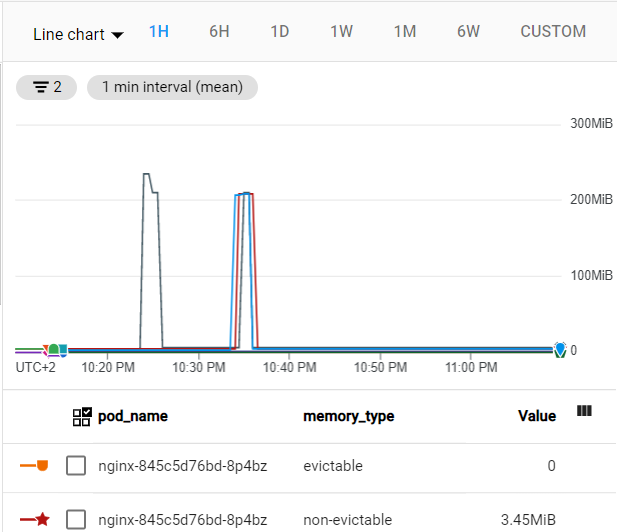
\includegraphics[scale=.7]{img/memory_spikes.png}
    \caption{Geheugen belasting nginx pods tot 200 MB}
\end{figure}

In vorig besproken chaos engineering tool Chaos Mesh kwam het Kubernetes object HorizontalPodAutoscaler alreeds aan bod in een soortgelijk experiment. Uitleg over wat een HPA doet kan men in subsectie \ref{subsec: HPA} terugvinden.   

Een vooraf gedefinieerde YAML-definitie kan men raadplegen in volgend Git repository bestand  \href{https://github.com/KenBruggeman/BP\textunderscore 21-22/blob/master/bachelorproef/docs/litmus%20experimenten/hpa.yaml}{Experiment 4 oplossing: hpa.yaml}

Gebruik volgend stappenplan om de HorizontalPodAutoscaler toe te passen:
\begin{enumerate}
    \item Plaats de inhoud van de YAML-definitie 'hpa.yaml' uit bovenstaande link in een nieuw bestand genaamd 'hpa.yaml' in de directory litmus-experiments. In dit bestand kan men zien dat de threshold ingesteld is op 100 MB en dat er mag geschaald worden tot zes pods indien nodig. Zodra de threshold overschreden wordt zullen nieuwe pods gecreëerd worden. Zie \ref{img:threshold} ter verduidelijking.
    \item Activeer de HorizontalPodAutoscaler m.b.v. commando {\bf kubectl apply -f hpa.yaml}.
    \item Herhaal experiment 4 via {\bf kubectl apply -f nginx-pod-memory-hog.yaml}.
\end{enumerate}    
  
Via k9s ziet men hoe drie nieuwe pods gecreëerd worden om de belasting mee te helpen opvangen.
Deze nieuwe nginx pods zullen gevrijwaard blijven van de geheugenbelasting die het lopende experiment veroorzaakt en dus niet belast worden zoals de vooraf bestaande nginx pods.  

\begin{figure}[h]
    \centering
    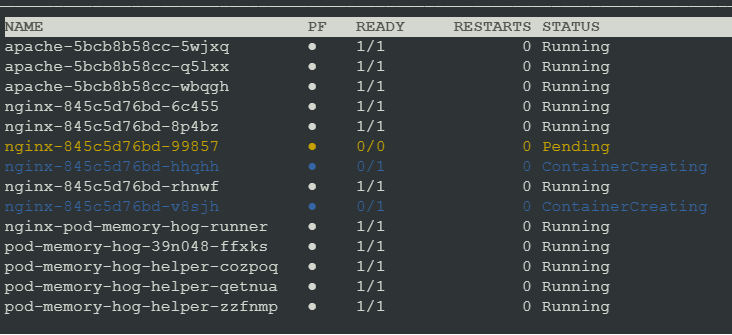
\includegraphics[scale=.9]{img/hpa_effect.png}
    \caption{HorizontalPodAutoscaler creëert drie nieuwe nginx pods}
    \label{img:threshold}
\end{figure}

\subsection{Experimenten uitvoeren via Litmus ChaosCenter}
\label{subsec:expchaoscenter}

Bovenstaande experimenten zijn allemaal tot nu toe uitgevoerd via de terminal. Hierdoor moet men echter verschillende manuele stappen doorlopen alvorens te kunnen overgaan tot de uitvoer van een experiment. Via de browser kan men deze experimenten ook uitvoeren in het Litmus ChaosCenter, die in een voorgaand hoofdstuk \ref{subsec:chaoscenter} alreeds werd opgezet. 

Ga via de browser naar Litmus ChaosCenter en vul de credentials in om toegang te krijgen. Gebruik volgend stappenplan om experiment 3 (= herhalende pod vernietiging met probe) te herhalen via deze GUI:
\begin{enumerate}
    \item Ga in het linkermenu naar {\bf Litmus Workflows} en klik vervolgens op 'Schedule a workflow'
    \item In tabblad {\bf Choose Agent}: selecteer de (enige) Self-Agent die hier aanwezig is en klik op Next. Een self-agent is een benaming voor de cluster waarop we het experiment willen uitvoeren.
    \item In tabblad {\bf Choose a workflow}: kies voor `Create a new workflow using the experiments from ChaosHubs` en klik op Next.
    \item In tabblad {\bf Workflow Settings}: Geef de workflow een naam naar wens (vb. iterated-podtato-head-pod-kill) en klik op Next.
    \item In tabblad {\bf Tune workflow}: kies rechtsboven voor `Add a new experiment`. Kies in de lijst die vervolgens getoond wordt voor `generic/pod-delete` en bevestig via Done.
    \item Men ziet de naam van het experiment in de workflow verschijnen. Rechts naast de naam klikt men het potlood aan om de nodige aanpassingen in te stellen.
    \item In sectie {\bf General}: verander niks en klik op Next.
    \item In sectie {\bf Target Application}:
        \begin{enumerate}
            \item open de dropdownlist `appns` (app namespace) en selecteer de namespace `demoapp2`, waar de podtato-head applicatie actief is.
            \item open de dropdownlist `applabel` en kies voor `app.kubernetes.io/name=podtato-head`.
            \item Ga verder door op Next te klikken.
        \end{enumerate}
    \item In sectie {\bf Define the steady state}:
        \begin{enumerate}
            \item kies voor `Add a new probe`.
            \item geef de probe een naam naar wens vb. application-access
            \item kies als probe type `http` m.a.w. bereikbaarheid van URL controleren
            \item kies als probe mode `Continuous` m.a.w. gedurende heel het experiment
            \item stel de {\bf Probe Properties} in m.a.w. hoe vaak gecontroleerd moet worden als de opgegeven URL bereikbaar is a.d.h.v. verschillende parameters.
            
            De Podtato-Head applicatie bevat meerdere pods waarvan één pod nl. 'podtato-head-entry' de toegang tot de applicatie voorziet via de Service LoadBalancer (of NodePort). Wanneer het experiment deze pod zou vernietigen kan de http-probe hierdoor falen aangezien de applicatie tijdelijk onbereikbaar wordt. Vandaar moet men rekening houden dat voldoende tijd ingesteld wordt bij 'interval' om de kans op slagen tijdens het opnieuw proberen van de probe te verhogen.  
            
            \item stel de {\bf Probe Details} in m.a.w. de URL van de PodTato-Head applicatie, hoe deze getest wordt nl. via een GET-request, hoelang het mag duren om de response te krijgen op deze request en welke HTTP status code terug verwacht wordt, in dit geval code 200 (OK).
            
            Een metric om de laadsnelheid van een pagina te volgen is de {\bf TTFB of time to first byte}. Men kan dit vooraf controleren door naar de applicatie te surfen, de Developer Tools (F12) te openen en naar tabblad Network te gaan. Daar voert men een reload uit via CTRL + F5 en kan men zien hoelang het duurt van request tot eerste byte van de response. \autocite{Mensink2022}
            
            \item Bevestig alle configuraties onderaan via Done.  
        \end{enumerate}
    \item In sectie {\bf Tune Experiment}:
        \begin{enumerate}
            \item stel 'Total chaos duration' in op 120 seconden m.a.w. experiment duurt 2 minuten
            \item stel 'Chaos interval' in op 10 m.a.w. elke 10 seconden wordt een pod verwijderd
            \item stel 'Force' in op false m.a.w. graceful termination \autocite{Dinesh2018a}
            \item Bevestig configuratie door op 'Finish' te klikken.
        \end{enumerate}  
    \item In sectie {\bf Advanced options to tune workflow}: activeer `Cleanup Chaos Workflow Pods` zodat na het uitvoeren van het experiment, de nodige helper pods ook terug verwijderd worden.
    Bevestig vervolgens via 'Save Changes'.
    \item Klik rechtsonderaan op Next om alle configuraties te bevestigen en naar het volgende tabblad te gaan.
    \item In tabblad {\bf Reliability Score}: staat standaard op 10, is niet van belang voor de uitvoer van experimenten. Klik op Next om door te gaan.
    \item In tabblad {\bf Choose a chaos schedule}: kies voor `Schedule now` en klik op Next. Men kan hier ook opteren een 'Recurring Schedule' te creëeren die het experiment op vaste tijdstippen vb. elk uur, elke dag, elke maand ... zal uitvoeren.
    \item In tabbled {\bf Summary}: Bevestig de configuratie rechtsonderaan via Finish. Bevestig nogmaals via `Go to workflow`.  
\end{enumerate}

De workflow start nu op waarvan het experiment slechts één specifiek onderdeel is. In de workflow zal men eerst het experiment (m.a.w. het object ChaosExperiment uit de ChaosHub) installeren alvorens de ChaosEngine (= de configuratie van het experiment) uit te voeren. Na de uitvoer van het experiment start het laatste onderdeel van de workflow nl. de toegebrachte chaos ongedaan maken.

Tijdens de uitvoer van het experiment kan men via de tool k9s zien dat er regelmatig pods van de podtato-head applicatie in de namespace litmusexperiments verwijderd worden. Doordat deze pods via een Deployment opgezet zijn zal de ReplicaSet er voor zorgen dat het gewenste aantal pods in de configuratie steeds gerespecteerd blijft. De http-probe zal controleren als de applicatie bereikbaar blijft gedurende het experiment.
 
\subsubsection{Workflow herhalen/aanpassen}

Wanneer men de configuratie van een uitgevoerde workflow wil aanpassen, of de workflow opnieuw wil uitvoeren, dan gaat men in het linkermenu bij Litmus Workflows naar het tabblad Scheduled.

Door uiterst rechts naast de workflow het menu te openen ziet men de optie **Rerun Schedule** om de workflow opnieuw uit te voeren.

Via de optie 'Save Template' kan men een wijziging aanbrengen aan de configuratie van de workflow. Hierbij wordt gevraagd een nieuwe workflow naam op te geven. Men kan een aanpassing namelijk NIET rechtstreeks uitvoeren in de bestaande workflow! De nieuwe aangepaste workflow zal men vervolgens aanspreken via optie 'Schedule a workflow'. In het tabblad {\bf Choose a workflow} kan men vervolgens kiezen voor 'Create a new workflow by cloning an existing workflow'. Daar zal de aangepaste versie van de bestaande workflow terug te vinden zijn. Aangezien alle configuraties alreeds opgenomen zijn in deze kan men direct doorgaan tot het uitvoeren van de aangepaste workflow. 

\subsubsection{Extra functionaliteit in Litmus ChaosCenter}

Andere Litmus experimenten die alreeds uitgevoerd werden in de terminal kunnen op soortgelijke manier via een workflow opgezet worden. Men kan zelfs verschillende experimenten gelijktijdig uitvoeren in een workflow via de knop {\bf Edit Sequence} in tabblad {\bf Tune Workflow} (zie stap 5 in bovenstaand stappenplan). 

In het linkermenu kan men bij {\bf Observability} o.a. statistieken raadplegen van alreeds uitgevoerde experimenten, een monitoring dashboard toevoegen in de GUI ...

Deze extra opties zijn niet verder onderzocht doordat meerdere experimenten gelijktijdig uitvoeren geen meerwaarde biedt in deze context, en een monitoring dashboard alreeds beschikbaar is via het Google Cloud Platform. 

\subsection{Conclusie Litmus}

Het installeren van Litmus verliep vlot via de package manager Helm. De documentatie mocht wel duidelijker zijn omtrent de minimum vereisten qua CPU en geheugen per node. Zo werd na eerste installatiepogingen duidelijk dat de Litmus pods vrij veel resources nodig hadden om operationeel te kunnen zijn.   

De verschillende objecten die Litmus gebruikt om een experiment op te zetten nl. ChaosExperiment, ChaosEngine, ServiceAccount, RBAC-regels ... maken deze chaos engineering tool vrij ingewikkeld om aan te leren. Ook is de documentatie die hulp kan bieden bij de experimenten soms moeilijk te vinden. 

Litmus experimenten opzetten via de terminal is vrij omslachtig. Men moet manueel de nodige experimenten vooraf installeren, de nodige permissies configureren, de ChaosEngine manueel opzetten ...
Ook wanneer een experiment niet naar wens verloopt en men dit vervolgens wil troubleshooten, moet men verschillende objecten analyseren vb. helper pods onderzoeken, uitvoer van chaosengine object bestuderen ... 

Bovenstaand proces wordt makkelijker wanneer experimenten opgezet worden via het Litmus ChaosCenter. Experimenten worden bij de start van een workflow steeds geïnstalleerd, men hoeft geen YAML-definitie op te stellen maar gewoon parameters te configureren, men kan indien nodig logs raadplegen na afloop van een experiment om troubleshooting eenvoudiger te maken ...

Litmus is een waardige tool om chaos experimenten uit te voeren op applicaties in een Kubernetes cluster, maar heeft een steile leercurve vooraleer men er daadwerkelijk mee aan de slag kan. De documentatie omtrent de installatie en het opzetten van experimenten is er wel, maar is te wijd verspreid wat de leercurve bemoeilijkt. Ook het hoge aantal resources die de Litmus pods nodig hebben in vergelijking met voorgaand onderzochte tool ChaosMesh kan als nadelig aanschouwd worden.   